
\chapter{Implementaci\'on}\label{sec:Implementacion}

\section{Introducci\'on}

En este cap\'{i}tulo se detalla la construcci\'{o}n y estructura del prototipo desarrollado, En las figuras ~\ref{fig:GimbalModel} y ~\ref{fig:GimbalViews}, podemos observar el dise\~{n}o 3D del prototipo realizado en el programa de modelado y simulaci\'{o}n mec\'{a}nica SolidWorks\textsuperscript{\textregistered}, mientras que en la fotograf\'{i}a de la figura ~\ref{fig:PrototipoTerminado} observamos el prototipo terminado. Este prototipo se realiz\'{o} en conjunto con el Instituto de Investagaci\'{o}n y Desarrollo Tecnol\'{o}gico de la Armada de M\'{e}xico (INIDETAM) durante una estancia de seis meses en las instalaciones del instituto. La construcci\'{o}n del prototipo se divide en tres aspectos claves, la mec\'{a}nica, la electr\'{o}nica y la programaci\'{o}n. La mec\'{a}nica y electr\'{o}nica del prototipo se basa en el desarrollo realizado por el INIDETAM  previo al inicio de este trabajo. El desarrollo previo al inicio de la tesis consiste en el dise\~{n}o mec\'{a}nico b\'{a}sico del sistema, la estructura de soporte y montaje, el tipo y m\'{e}todo de transmisi\'{o}n de potencia de los motores a los eslabones interno y externo del sistema, la selecci\'{o}n del material as\'{i} como el maquinado. Por el lado del desarrollo electr\'{o}nico, en el instituto se dise\~{n}aron dos tarjetas electr\'{o}nicas dedicadas para el control del sistema, una para el control del movimiento de pan y el otro para el movimiento en tilt estas tarjetas cuentan con todos los dispositivos necesarios para el procesamiento y comunicaci\'{o}n del sistema, as\'{i} como para el control de los motores y la c\'{a}mara. Para la detecci\'{o}n de l\'{i}mites f\'{i}sicos del sistema, en el instituto se desarrollaron sensores de l\'{i}mite magn\'{e}ticos, los cuales no funcionaron en la implementaci\'{o}n por lo que tuvieron que ser redise\~{n}ados.          

\begin{figure}[H]
\centering 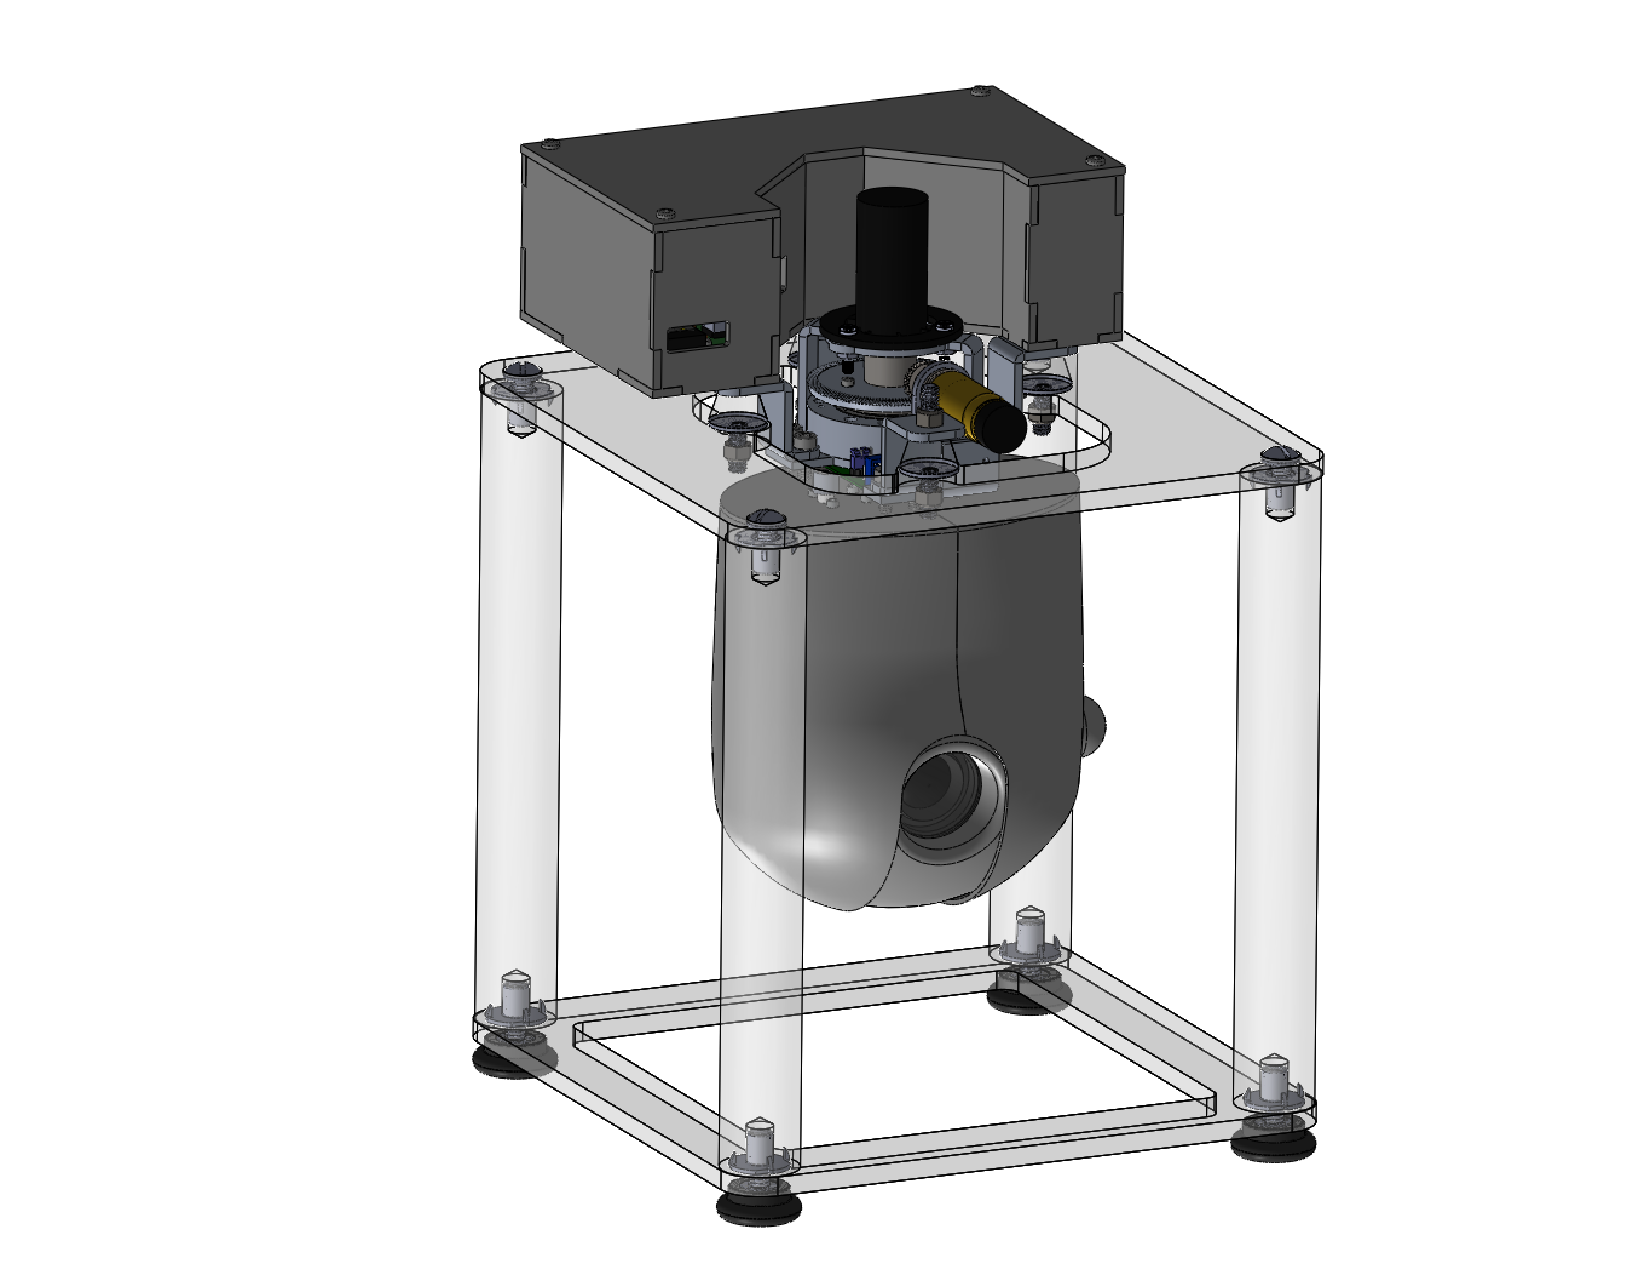
\includegraphics[scale=0.45]{img/Gimbal2.pdf}
%trim = izquierda abajo derecha arriba [scale=0.5,trim = 40mm 30mm 110mm 15mm, clip]
\caption{Modelo 3D del Prototipo de C\'{a}mara Giroestablizada}
\label{fig:GimbalModel}
\end{figure}

La programaci\'{o}n del microcontrolador se realiz\'{o} utilizando los MPLAB\textsuperscript{\textregistered} Device Blocks for Simulink\textsuperscript{\textregistered}. Esta herramienta creada por la empresa Microchip\textsuperscript{\textregistered}, permite utilizar el entorno de Simulink\textsuperscript{\textregistered} para la programaci\'{o}n de los microcontroladores Microchip\textsuperscript{\textregistered} de las familias dsPIC\textsuperscript{\textregistered}30 y dsPIC\textsuperscript{\textregistered}33. Esta herramienta permite la configuraci\'{o}n de los perif\'{e}ricos del microcontrolador a trav\'{e}s de bloques de Simulink, lo cual facilita en gran medida las aplicaciones. Tambi\'{e}n es posible a\~{n}adir bloques que ejecuten c\'{o}digo en lenguaje C, brindando la oportunidad que crear funciones personalizadas y tener acceso a caracter\'{i}sticas de los dsPIC\textsuperscript{\textregistered} no disponibles con los bloques predeterminados incluidos.  


\begin{figure}[H]
\centering 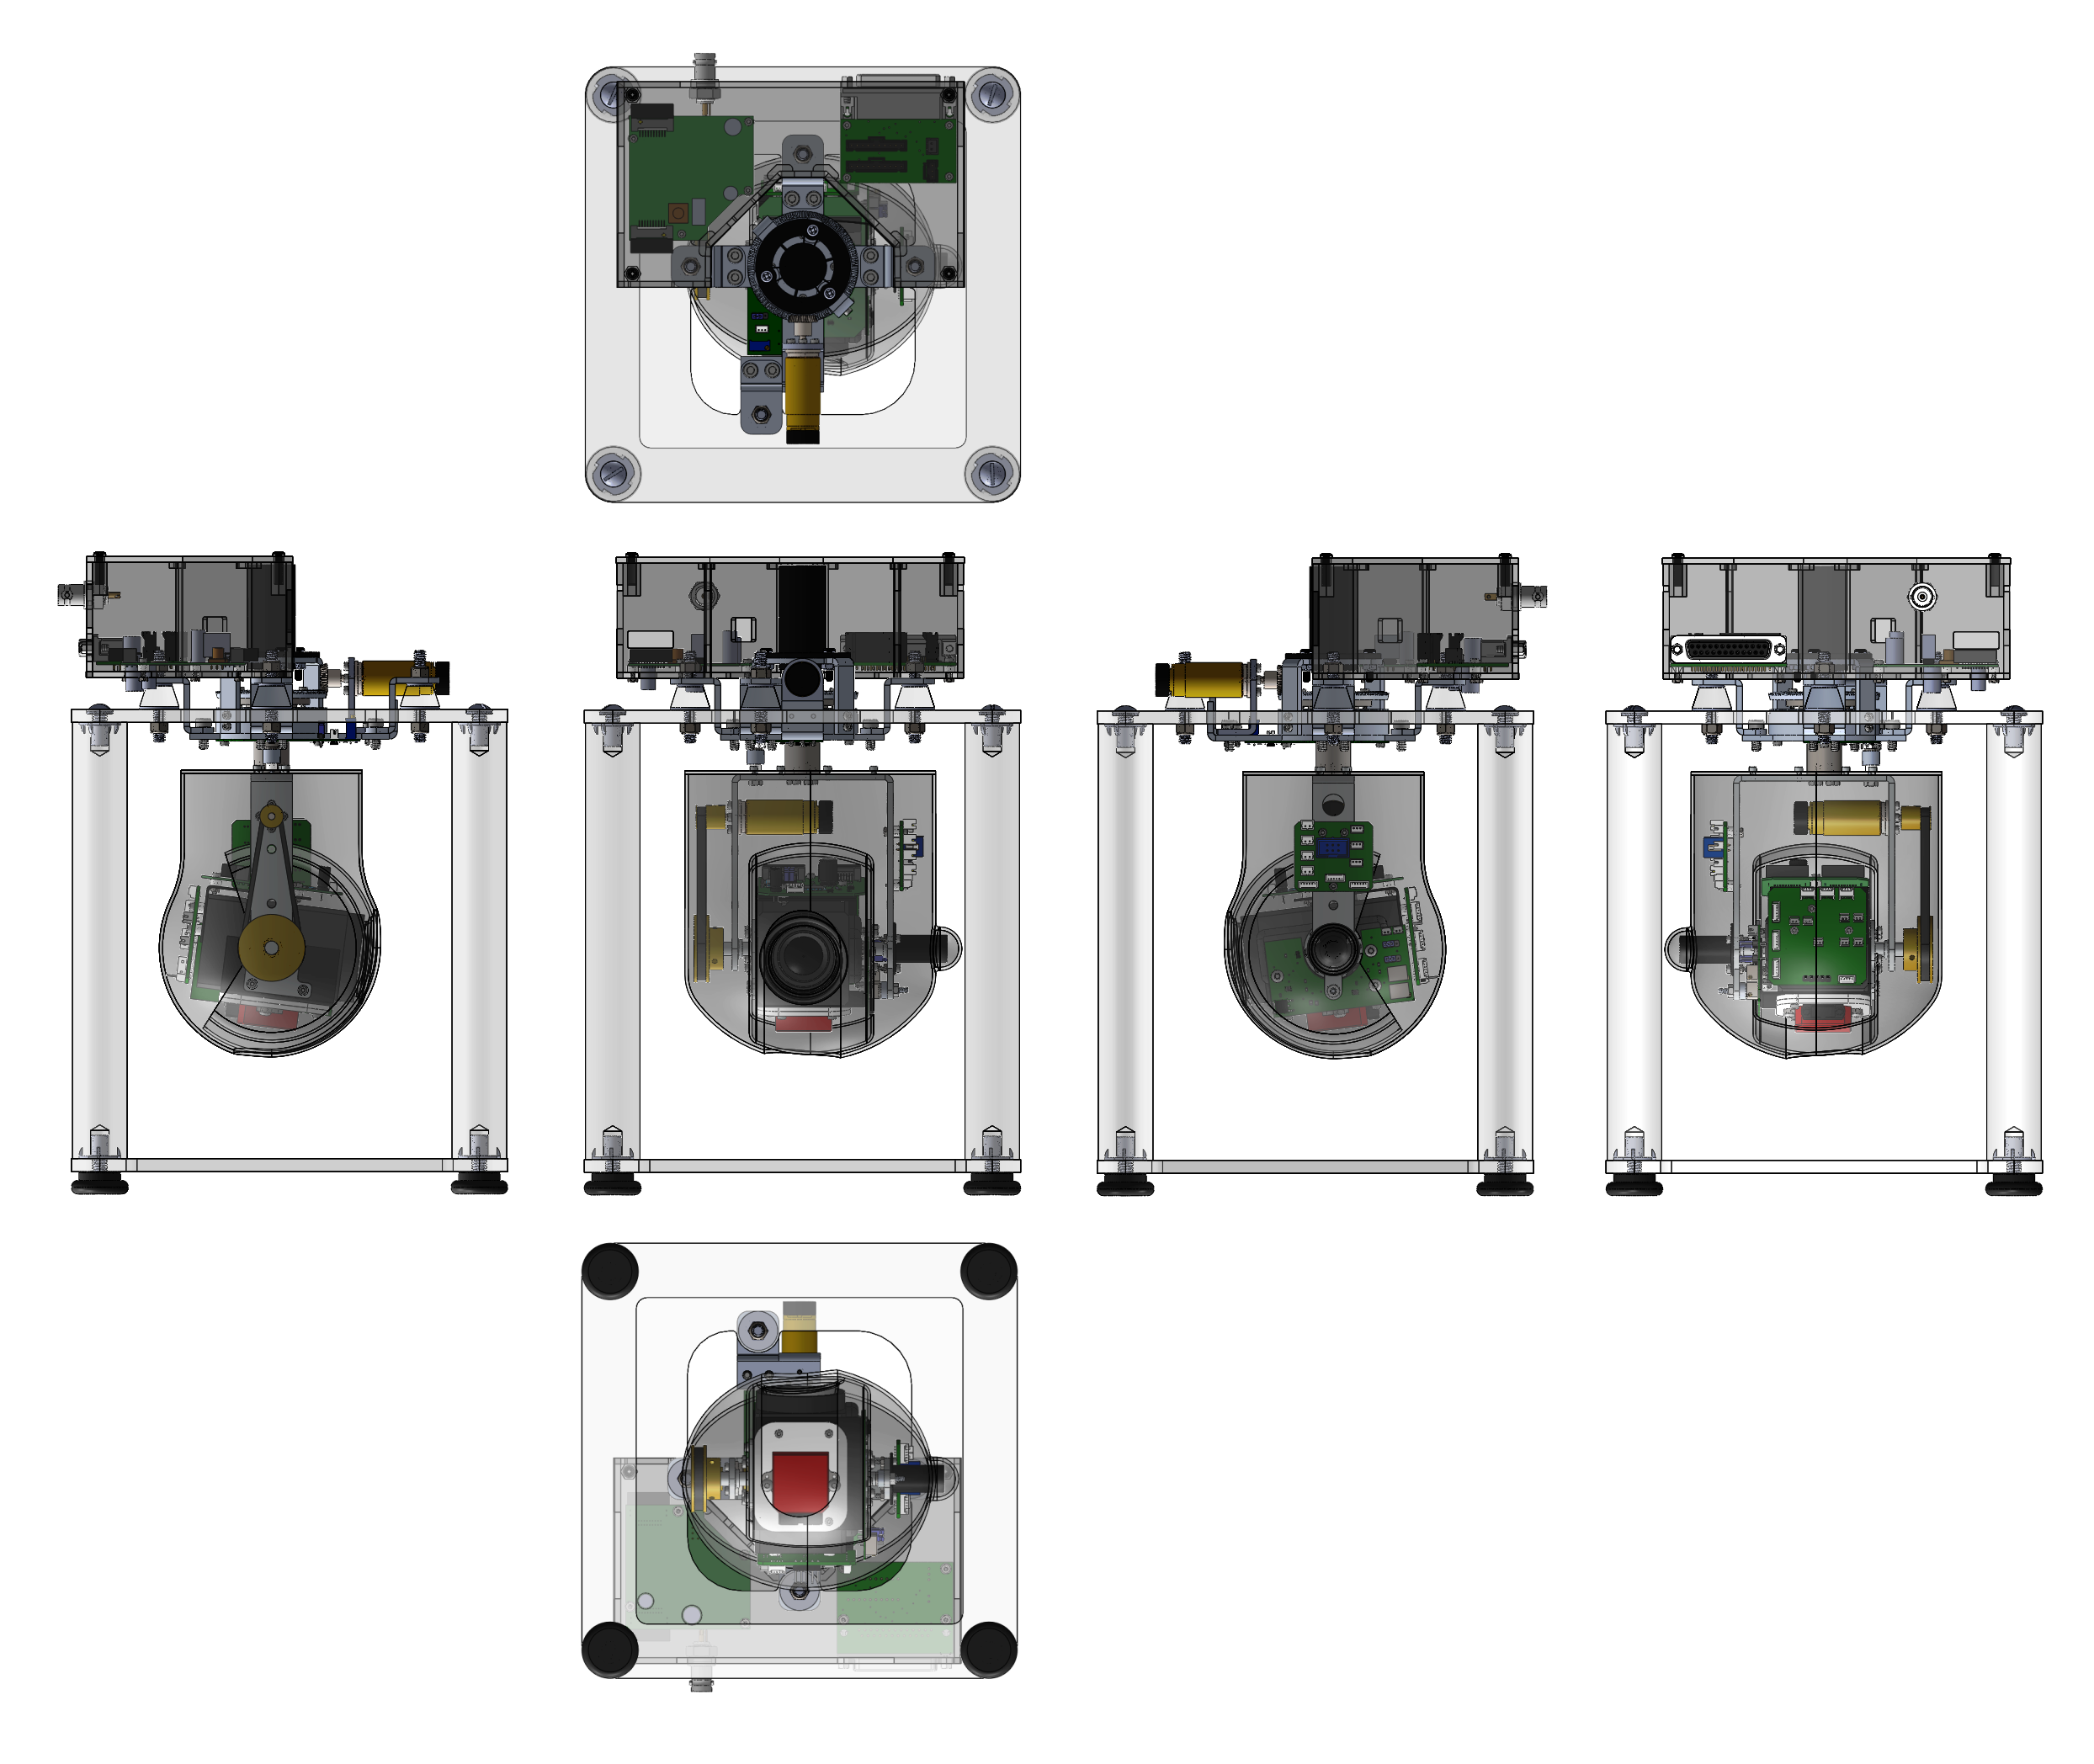
\includegraphics[scale=0.25]{img/GimbalViews.png}
%trim = izquierda abajo derecha arriba [scale=0.5,trim = 40mm 30mm 110mm 15mm, clip]
\caption{Vistas del Modelo 3D del Prototipo de C\'{a}mara Giroestablizada}%Esta es la l\'{i}nea para el pie de figura
\label{fig:GimbalViews}%esta es la etiqueta para referenciar en el texto la figura: ...como se aprecia de la Figura \ref{termopar}...
\end{figure}

Fueron necesarias modificaciones en el dise\~{n}o mec\'{a}nico original para mejorar las capacidades del sistema gimbal, una modificaci\'{o}n clave fue la instalaci\'{o}n de un slip ring\footnote{Un slip ring es un dispositivo electromec\'{a}nico que permite la transmici\'{o}n de energ\'{i}a o se\~{n}ales el\'{e}ctricas de una estructura estacionaria a una rotativa} en el eslab\'{o}n interno lo cual permite un giro de 360 grados y elimina las limitaciones causadas por los cables, derivada de esta modificaci\'{o}n tuvieron que dise\~{n}arse dos placas electr\'{o}nicas para la distribuci\'{o}n de se\~{n}ales entre la tarjeta de control en tilt y la tarjeta principal, ya que las conexiones disponibles en el slip ring eran menores de las necesarias. Finalmente para la f\'{a}cil manipulaci\'{o}n del sistema fue necesario dise\~{n}ar una base a la medida para el prototipo, la cual podemos ver en la figura ~\ref{fig:PrototipoTerminado}, La base est\'{a} fabricada en acr\'{i}lico de seis mil\'{i}metros cortado con l\'{a}ser y barra de una pulgada de di\'{a}metro, igualmente de acr\'{i}lico para los postes los cuales tienen injertos roscados de 1/4 de pulgada para poder ensamblarse, estos fueron insertados en la barra calentado los injertos de acero y posteriormente los postes fueron devastados en torno para que tuvieran una medida precisa. Esta base se dise\~{n}\'{o} y construy\'{o} con el fin de  manipular y almacenar del prototipo de forma segura.

\begin{figure}[H]
\centering 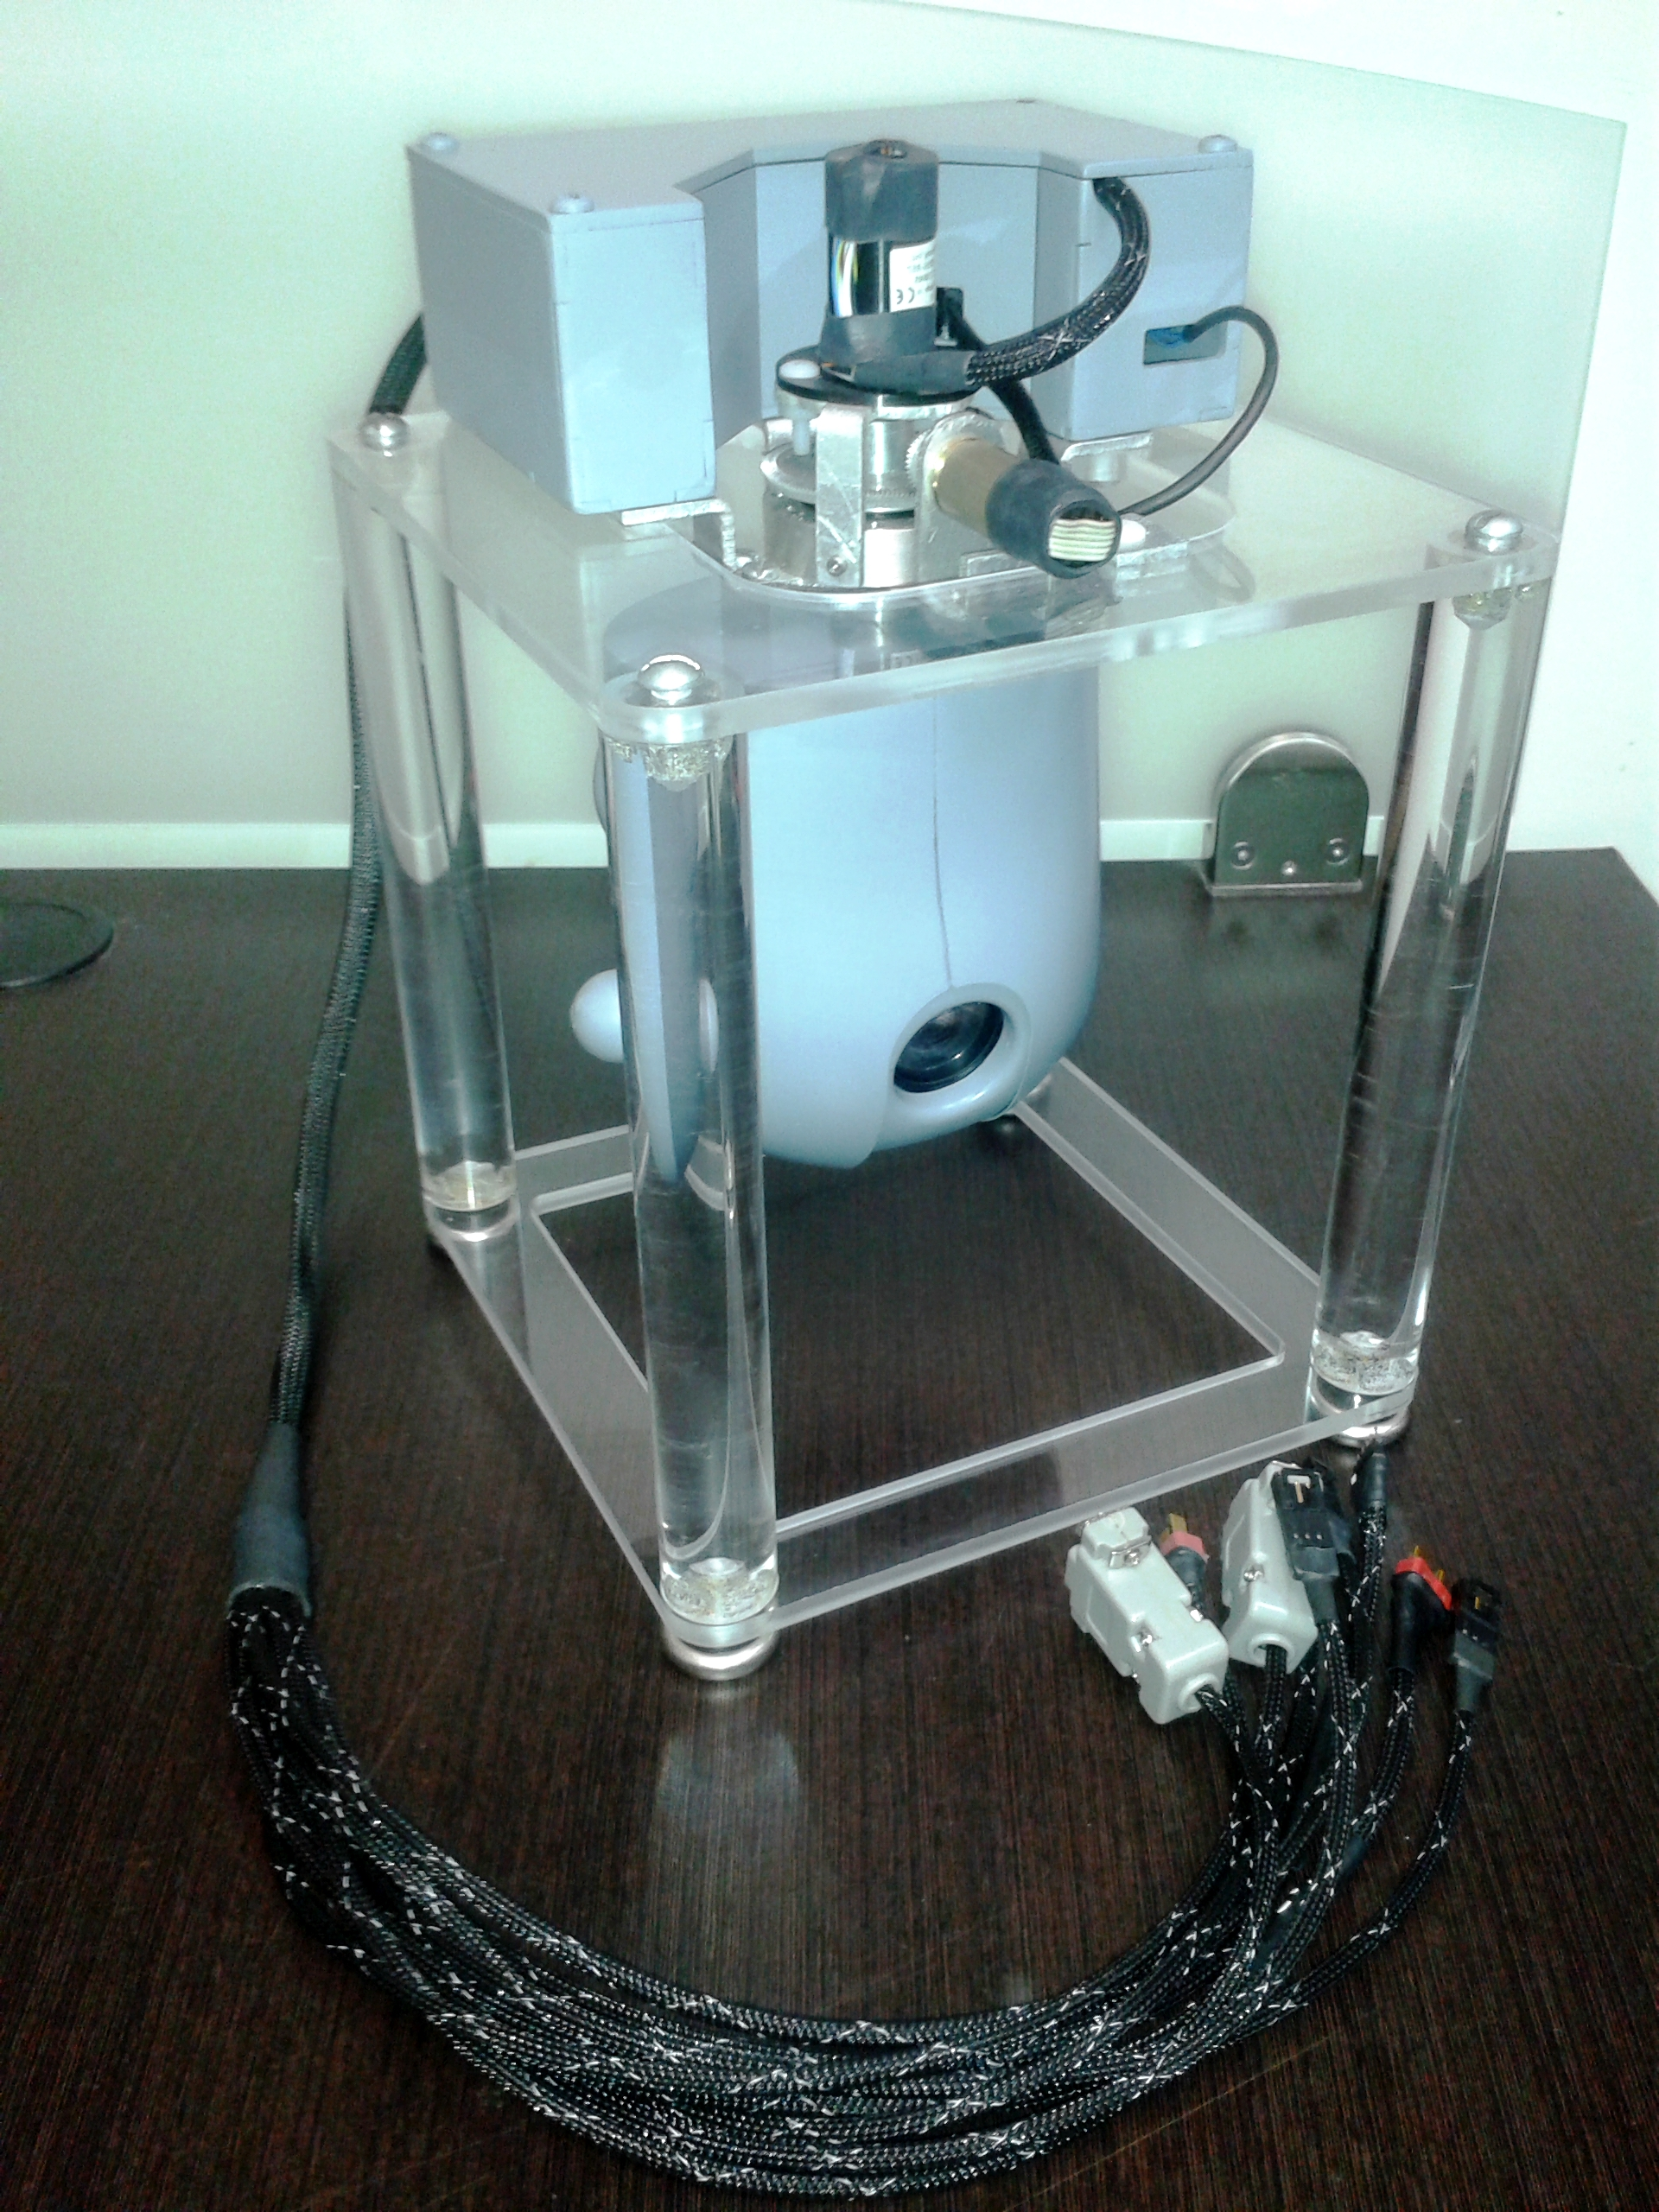
\includegraphics[scale=0.11]{img/PrototipoTerminado.jpg}
%trim = izquierda abajo derecha arriba [scale=0.5,trim = 40mm 30mm 110mm 15mm, clip]
\caption{Prototipo Terminado}
\label{fig:PrototipoTerminado}
\end{figure} 

\section{Electr\'onica}

\subsection{Tarjetas de Control}

Las tarjetas principales de control para el sistema fueron desarrolladas por el Dr. Mariano Lizarraga en el laboratorio de veh\'{i}culos aut\'{o}nomos del INIDETAM previo al inicio de esta tesis, podemos apreciar estas tarjetas en la figura ~\ref{fig:MainBoards}, la tarjeta del lado izquierdo es la \textit{"Main Board"} o tarjeta principal de control, la tarjeta de la derecha es la \textit{"Tilt Board"} o tarjeta de control de tilt. Sin embargo no se desarroll\'{o} el firmware\footnote{El firmware es un bloque de instrucciones de m\'{a}quina para prop\'{o}sitos espec\'{i}ficos, grabado en un chip, que establece la l\'{o}gica de m\'{a}s bajo nivel que controla los circuitos electr\'{o}nicos de un dispositivo y es el encargado de controlarlo para ejecutar correctamente las instrucciones externas} necesario para su funcionamiento, \'{u}nicamente se realiz\'{o} la programaci\'{o}n de controladores simples para algunos de sus perif\'{e}ricos. Por lo que esa tarea tuvo que llevarse a cabo como parte de esta tesis, este desarrollo se trata a detalle en la secci\'{o}n ~\ref{sec:Programacion}, en donde se describe el procedimiento y m\'{e}todo de programaci\'{o}n. 

\begin{figure}[H]
\centering
      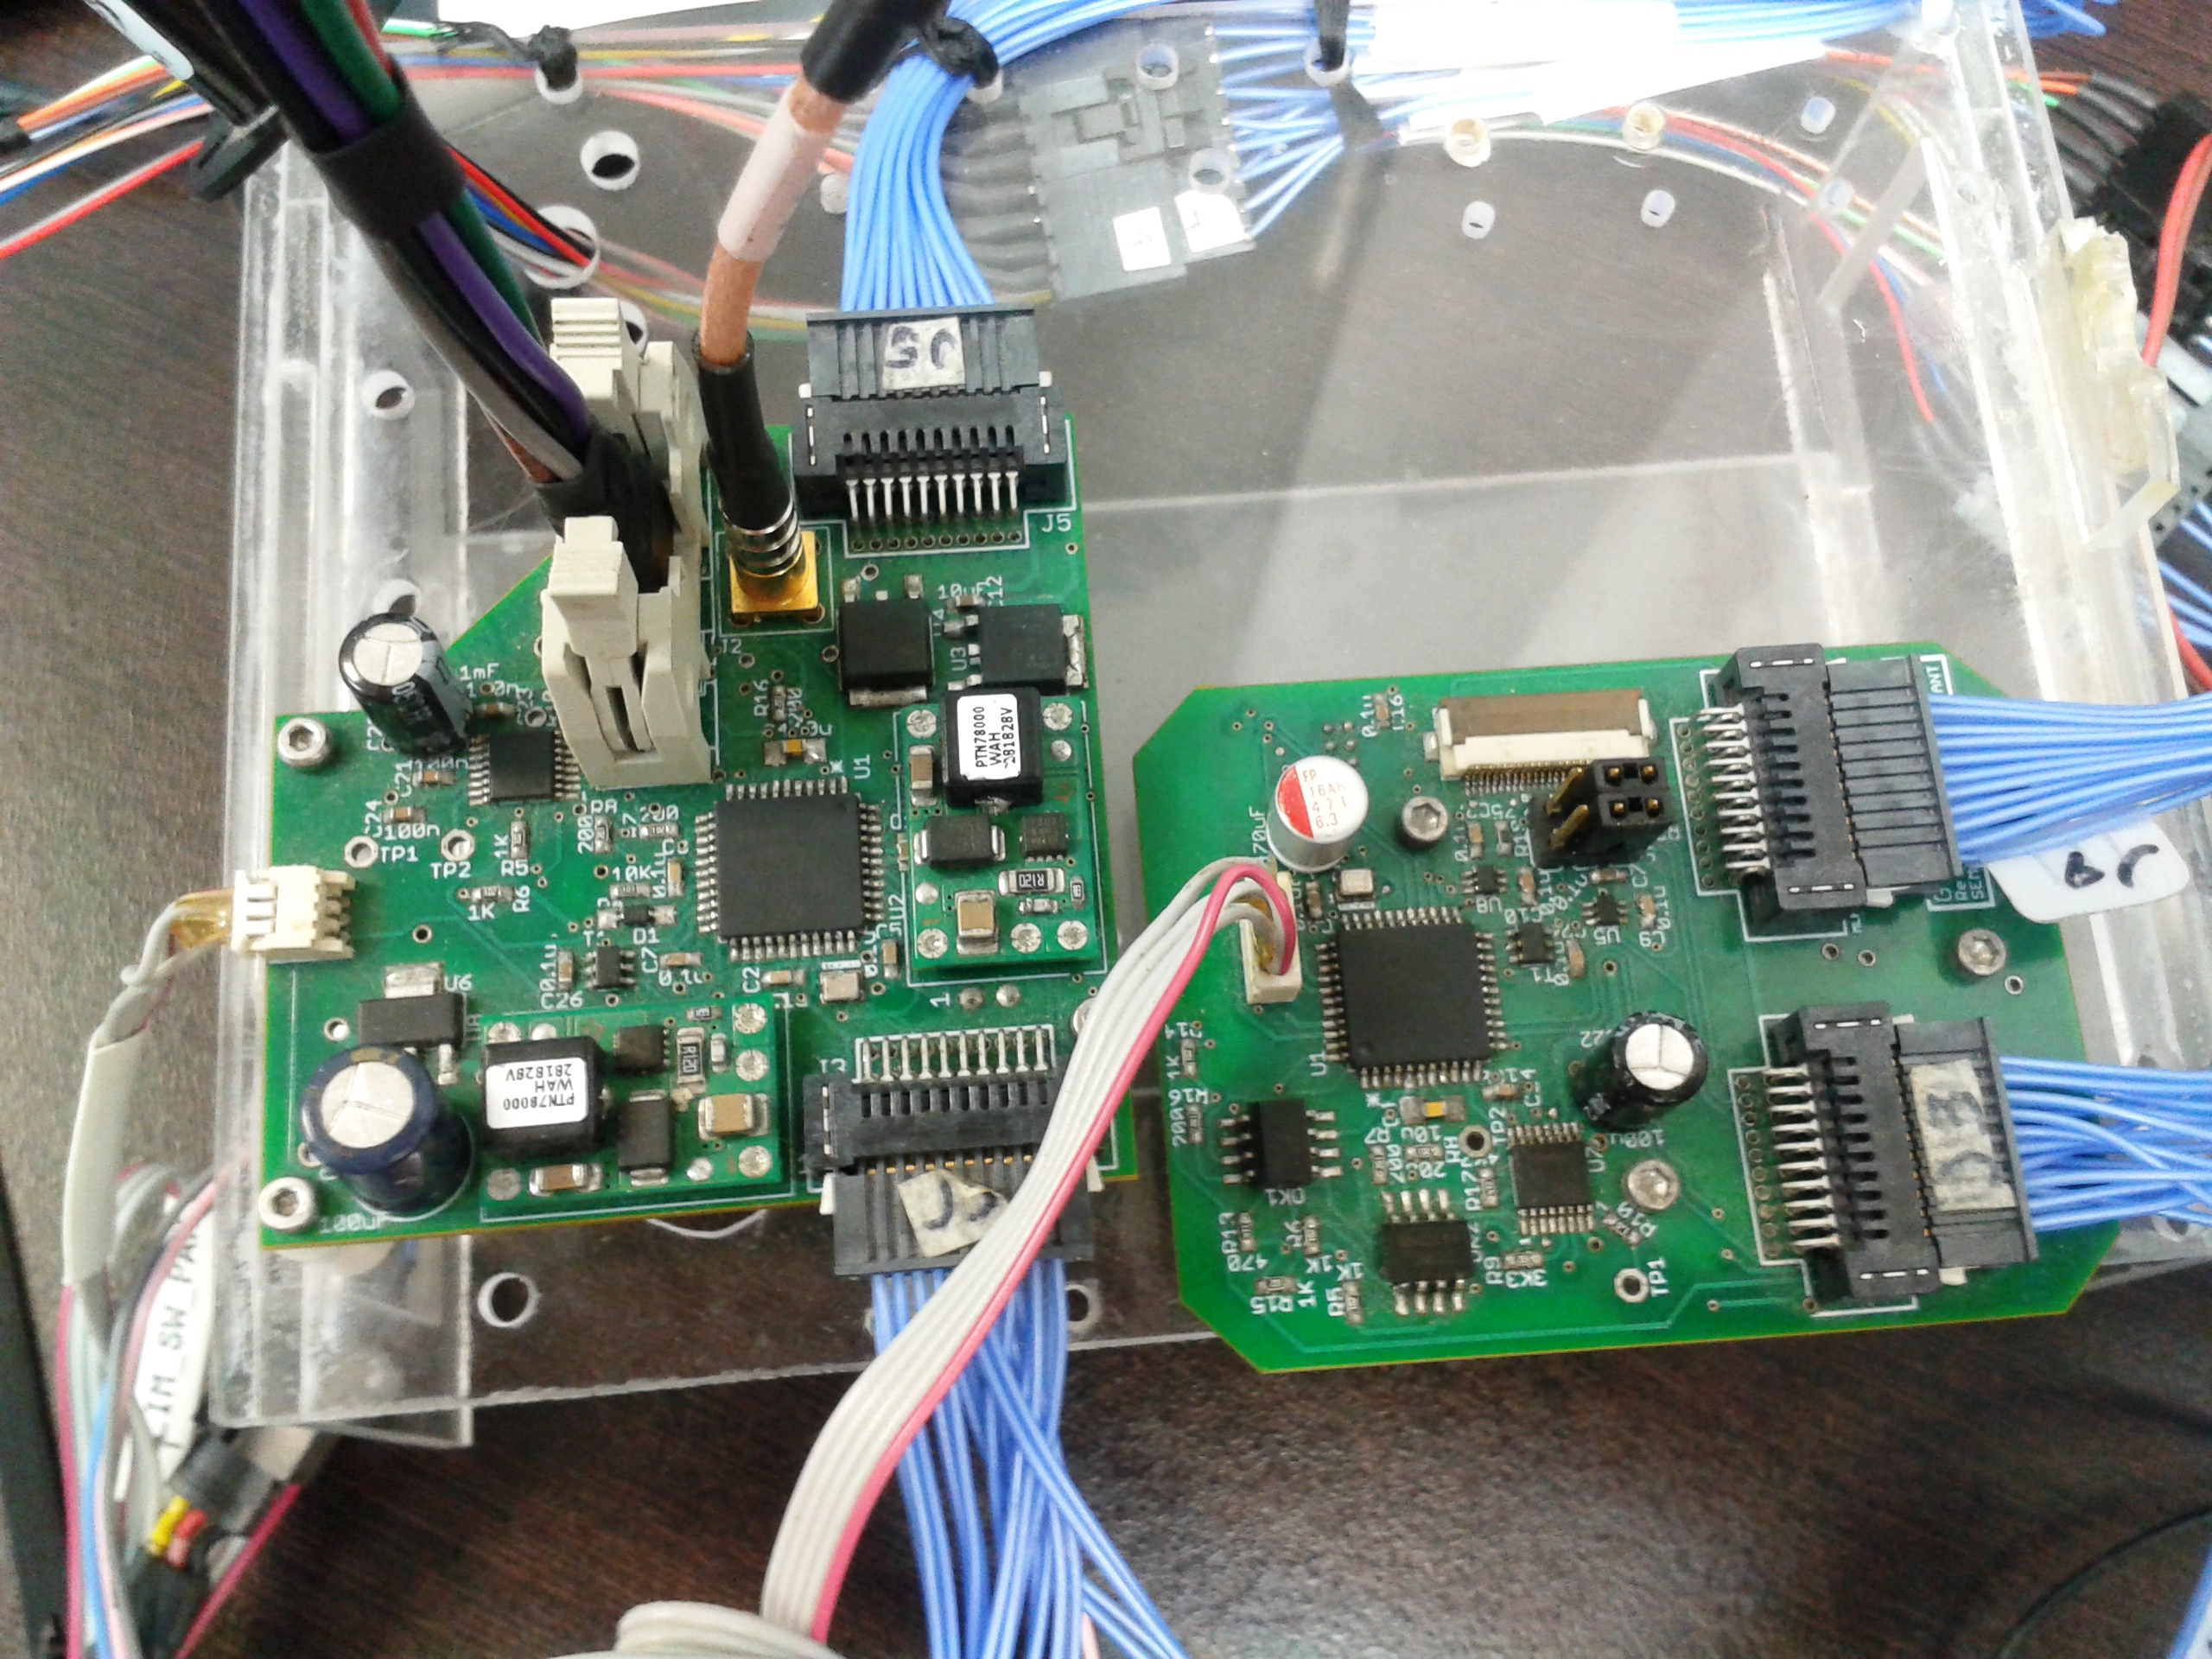
\includegraphics[scale=0.1]{img/Mainboards.jpg}
      \caption{Tarjetas Principales de Control del Sistema Montadas en el Banco de Pruebas}
      \label{fig:MainBoards}
\end{figure} 

La unidad de procesamiento central con el que cuentan estas tarjetas es un dsPIC33 de 16 bits. Estas tarjetas cuentan con todos los dispositivos electr\'{o}nicos necesarios para el control del sistema y a continuaci\'{o}n se describen sus caracter\'{i}sticas:\newline
\begin{large}
\textbf{Main Board} 
\end{large}

\begin{itemize}
    \item Procesador dsPIC33FJ128MC804 de 16 bits.
    \item Oscilador externo de 20 MHz.
    \item Transceptor de Bus CAN.
    \item Transceptor Serial RS232.
    \item Modulo de control para un encoder de cuadratura.
    \item Regulador interno de 24 v a 12 v para alimentaci\'{o}n de elementos de potencia.
    \item Reguladores internos de 12 v a 7 v, 5 v y 3.3 v para alimentaci\'{o}n de control.
    \item Salida regulada a 12 v y 7v.
    \item Driver para motor DC Texas Instruments\textsuperscript{\textregistered} DRV8801.
    \item Optoacoplamiento para aislamiento de la potencia de la l\'{o}gica de control.
    \item Sensor de Temperatura digital de 12 bits SPI.
    \item Conectores Samtec\textsuperscript{\textregistered} TFM-110-01-L-D para perif\'{e}ricos.
    \item Conector de v\'{i}deo Farnell\textsuperscript{\textregistered} MCX7-JPH-ST-TH1.
    \item Conexi\'{o}n a entrada digital para sensor de l\'{i}mite. 
    \item Programaci\'{o}n ICSP\footnote{Siglas para \textit{In-Circuit Serial Programming}, es la capacidad de algunos dispositivos l\'{o}gicos programables, microcontroladores y otros circuitos electr\'{o}nicos, de ser programados mientras est\'{a}n instalados en un sistema completo.}. 
\end{itemize}

\begin{large}
\textbf{Tilt Board} 
\end{large}

\begin{itemize}
    \item Procesador dsPIC33FJ128MC804 de 16 bits.
    \item Oscilador externo de 20 MHz.
    \item Dos m\'{o}dulos de comunicaci\'{o}n serial a 3.3 v.
    \item Modulo de control para un encoder de cuadratura.
    \item Dos conexi\'{o}n a entradas digitals para sensores de l\'{i}mite. 
    \item Reguladores internos de 7 v a 5v y 3.3v para alimentaci\'{o}n de control.
    \item Supresor de voltajes transitorios.
    \item Driver para motor DC Texas Instruments\textsuperscript{\textregistered} DRV8801.
    \item Optoacoplamiento para aislamiento de la potencia de la l\'{o}gica de control.
    \item Sensor de Temperatura digital de 12 bits SPI.
    \item Conectores Samtec\textsuperscript{\textregistered} TFM-110-01-L-D para perif\'{e}ricos.
    \item Conector tipo FFC de 0.5mm y 24 posiciones para interfaz con la c\'{a}mara SONY\textsuperscript{\textregistered} FCB-H11. 
    \item On-Screen Display\footnote{Es una imagen superpuesta sobre la pantalla de v\'{i}deo para mostrar informaci\'{o}n adicional.}.
    \item Programaci\'{o}n ICSP  
    \item Selector de l\'{i}nea para depuraci\'{o}n. 
    \item Capacidad para recepci\'{o}n de dos canales de v\'{i}deo con selector digital.
\end{itemize}


\subsection{C\'{a}mara}

La c\'{a}mara utilizada es la FCB-H11 de SONY\textsuperscript{\textregistered}, figura ~\ref{fig:Camara}, la cual es una c\'{a}mara de bloque de alta definici\'{o}n compatible con ocho formatos diferentes de v\'{i}deo que se muestran en la tabla ~\ref{Table:VideoFormat}, incluyendo el formato Full HD (1080i), que es equivalente a una se\~{n}al est\'{a}ndar de HD-TV. Las salidas de v\'{i}deo que maneja la c\'{a}mara son VBS\footnote{El v\'{i}deo compuesto es una se\~{n}al anal\'{o}gica de transmisi\'{o}n de v\'{i}deo en la que se codifica la imagen en sus diferentes componentes de luz y color a\~{n}adiendo los sincronismos necesarios para su posterior reconstrucci\'{o}n.} y Y/C\footnote{V\'{i}deo separado o s-video, es un tipo de se\~{n}al anal\'{o}gica de v\'{i}deo, tiene m\'{a}s calidad que el v\'{i}deo compuesto puesto que se separa la informaci\'{o}n del brillo y del color, mientras que en el v\'{i}deo compuesto se encuentran juntas.} para SD\footnote{Definici\'{o}n est\'{a}ndar, es la resoluci\'{o}n de v\'{i}deo dominante desde el origen de la TV hasta la aparici\'{o}n de la alta definici\'{o}n. El sistema est\'{a} alrededor de una resoluci\'{o}n de 500 l\'{i}neas horizontales.}  y componente anal\'{o}gico\footnote{V\'{i}deo por componentes es un t\'{e}rmino referido a la divisi\'{o}n de una se\~{n}al de v\'{i}deo en dos o m\'{a}s canales de componentes.} para HD\footnote{Alta definici\'{o}n, es un sistema de imagen, v\'{i}deo y/o sonido con mayor resoluci\'{o}n que la definici\'{o}n est\'{a}ndar, alcanzando resoluciones de 1280x720 p\'{i}xeles y 1920x1080 p\'{i}xeles.}. La c\'{a}mara est\'{a} equipada con un lente de zoom \'{o}ptico de enfoque autom\'{a}tico 10x y el zoom digital de 12x permite un zoom de hasta 120x, combinado con el zoom \'{o}ptico. 

\begin{figure}[H]
\centering 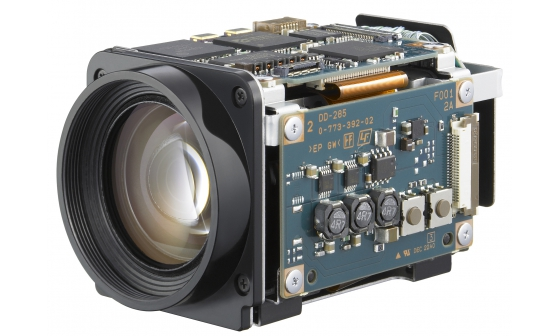
\includegraphics[scale=0.5]{img/Camara.jpeg}
\caption{SONY\textsuperscript{\textregistered} FCB-H11}
\label{fig:Camara}
\end{figure} 

La c\'{a}mara esta equipada con un filtro de infrarrojos dise\~{n}ado para reflejar o bloquear las longitudes de onda infrarroja dejando pasar \'{u}nicamente la luz del espectro visible. Este filtro puede ser desacoplado para incrementar la sensibilidad en ambientes de poca luz, a esta funci\'{o}n se le denomina Infrared Cutfilter Removal (ICR), El ICR se acoplar\'{a} autom\'{a}ticamente dependiendo de la luz ambiental, permitiendo a la c\'{a}mara ser efectiva en ambientes diurnos y nocturnos.

\begin{table}[h]
\caption{Formatos de V\'{i}deo de la C\'{a}mara FCB-H11}
\label{Table:VideoFormat}
\begin{center}
\begin{tabular}{ |l|l|l| }
\hline
\multicolumn{2}{ |c| }{Formatos de V\'{i}deo Soportados} \\
\hline
Tipo & Formato\\ \hline
\multirow{4}{*}{HD} 
 & 1080i/59.94\\
 & 1080i/50\\
 & 720p/59.94\\
 & 720p/50\\ 
 \hline
\multirow{4}{*}{SD} 
 & NTSC\footnotemark{}(Crop)\\
 & NTSC(squeeze)\\
 & PAL\footnotemark{}(Crop)\\ 
 & PAL(Squeeze)\\ 
\hline
\end{tabular}
\end{center}
\end{table}

\addtocounter{footnote}{-2}
\stepcounter{footnote}\footnotetext{Llamado as\'{i} por las siglas de \textit{National Television System Committee}. Es un sistema de codificaci\'{o}n utilizado para la transmisi\'{o}n de sistemas de televisi\'{o}n anal\'{o}gica, que consiste en 29.97 cuadros de v\'{i}deo por segundo con exploraci\'{o}n entrelazada.}
\stepcounter{footnote}\footnotetext{Sigla de \textit{Phase Alternating Line}. Es un sistema de codificaci\'{o}n utilizado para la transmisi\'{o}n de sistemas de televisi\'{o}n anal\'{o}gica en la que primero se exploran las l\'{i}neas impares y luego las pares.}

La c\'{a}mara utiliza el protocolo de comunicaciones VISCA, de sus siglas en ingl\'{e}s \textit{Video System Control Architecture}, el cual es un protocolo profesional para c\'{a}maras de vigilancia basado en RS232 con paquetes de los 3 a los 16 bytes desarrollado por SONY\textsuperscript{\textregistered}, el cual permite controlar la c\'{a}mara desde una computadora. Es posible seleccionar un amplio rango de velocidades de comunicaci\'{o}n de entre los 9600 bps, 19200 bps, o 38400 bps. Esto permite controlar la c\'{a}mara remotamente a una alta velocidad de comunicaci\'{o}n. La c\'{a}mara incluye la funci\'{o}n de posici\'{o}n de preajuste, lo que le permite guardar hasta seis diferentes configuraciones de las condiciones de captura de la c\'{a}mara, para poder elegir el comportamiento de la c\'{a}mara al encenderse. 

\subsection{Unidad de Medici\'{o}n Inercial}

La unidad de medici\'{o}n inercial (IMU) por sus siglas en ingl\'{e}s utilizada es la \textit{VN-100 Rugged} de VectorNav\textsuperscript{\textregistered}, figura ~\ref{fig:IMU}, que consiste en sensor VN-100 el cual tiene un CPU de 32 bits y varios sensores de estado s\'{o}lido integrados; un aceler\'{o}metro de tres ejes, un giroscopio de tres ejes, un magnet\'{o}metro de tres ejes y un sensor barom\'{e}trico de presi\'{o}n. Tiene una carcasa robusta de aluminio de alta precision de 36 x 33 x 9 mm con un conector de 10 pines y dos interfaces de comunicaci\'{o}n serial f\'{i}sicamente separadas RS232. 

\begin{figure}[H]
\centering 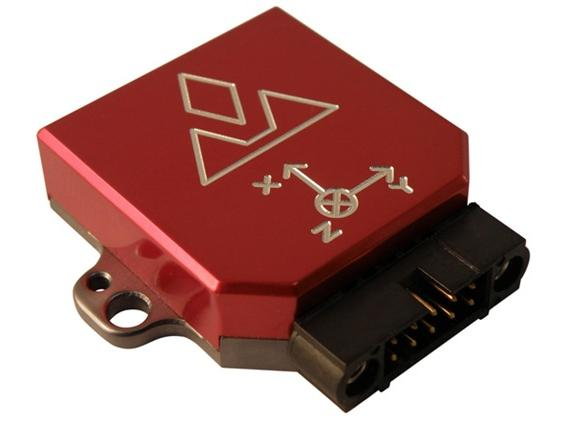
\includegraphics[scale=0.4]{img/VN100.jpg}
\caption{Central Inercial VectorNav\textsuperscript{\textregistered}}
\label{fig:IMU}
\end{figure} 

La arquitectura de software interna del VN-100 consiste en cuatro subsistemas separados. Estos subsistemas son la IMU, el NavState, el NavFilter y la interfase de comunicaciones. El subsistema de la IMU se ejecuta a la velocidad m\'{a}s alta del sistema (800Hz), este es el subsistema responsable de recolectar las mediciones brutas, aplicar calibraciones a las mediciones, aplicar una rotaci\'{o}n al marco de referencia y opcionalmente filtrar la se\~{n}al individual de cada sensor. El subsistema NavState, genera un flujo de datos continuo producido por el algoritmo de estimaci\'{o}n de la orientaci\'{o}n el cual es un filtro de Kalman extendido basado en quaterniones que provee un rango de movimiento completo de 360 grados y puede configurarse a una velocidad m\'{a}xima de 400Hz. El subsistema NavFilter consiste en un VPE\footnote{Son las siglas de \textit{Vector Processing Engine}. Un procesador vectorial es un dise\~{n}o de CPU capaz de ejecutar operaciones matem\'{a}ticas sobre m\'{u}ltiples datos de forma simult\'{a}nea.} y una variedad de filtros Kalman que se ejecutan a una velocidad menor que el subsistema NavState (200Hz). La interfase de comunicaciones que provee el sensor VN-100 consiste en dos interfases seriales UART\footnote{Siglas en ingl\'{e}s para Transmisor-Receptor As\'{i}ncrono Universal, es el dispositivo que controla los puertos y dispositivos serie.} bidireccionales f\'{i}sicamente separadas y un bus SPI. Cada interfaz UART soporta velocidades desde los 9600 bps hasta un m\'{a}ximo de 921600 bps. Las interfaces UART trabajan a voltajes TTL\footnote{Siglas en ingl\'{e}s de l\'{o}gica transistor a transistor. Es una tecnolog\'{i}a de construcci\'{o}n de circuitos electr\'{o}nicos digitales en que  los elementos de entrada y salida del dispositivo son transistores bipolares.} de 3 v, sin embargo el VN-100 Rugged tiene un tranceptor que permite usar una interfaz serial a voltajes serial RS232 est\'{a}ndar. El protocolo de comunicaci\'{o}n usado por el VN-100 puede configurarse para ser un protocolo binario o ASCII\footnote{Acr\'{o}nimo del ingl\'{e}s para C\'{o}digo Est\'{a}ndar Estadounidense para el Intercambio de Informaci\'{o}n, es un c\'{o}digo de caracteres basado en el alfabeto latino, tal como se usa en ingl\'{e}s moderno.} basado en comandos y polling\footnote{Es la operaci\'{o}n de consulta constante, generalmente hacia un dispositivo de hardware, para crear una actividad sincr\'{o}nica sin el uso de interrupciones.} de registros. El protocolo ASCII es muy similar al protocolo NMEA 0183 ampliamente utilizado por la mayor\'{i}a de los receptores GPS y consiste par\'{a}metros separados por una coma impresos en texto legible por un humano. En la figura ~\ref{fig:VN100Responce} se muestra un ejemplo del comando de solicitud y respuesta del VN-100 en protocolo ASCII.

\begin{figure}[H]
\centering 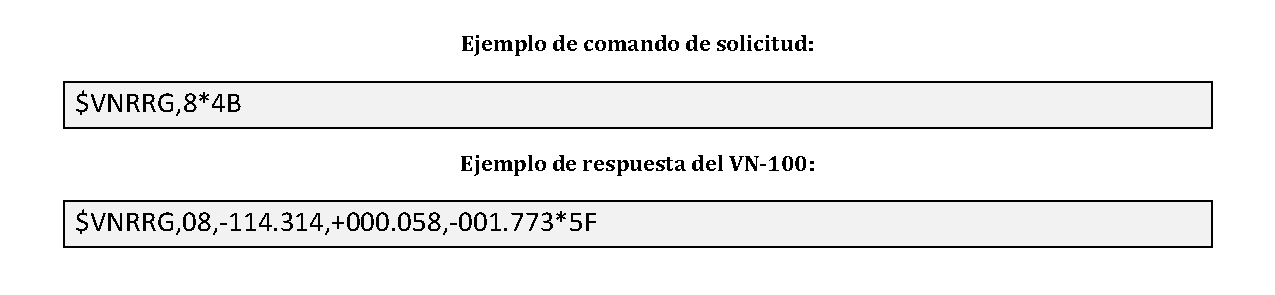
\includegraphics[scale=0.8]{img/VN100Responce.pdf}
\caption{Ejemplo del Protocolo de Comunicaci\'{o}n del VN-100}
\label{fig:VN100Responce}
\end{figure} 

\subsection{Motor}

El motor utilizado para el control de ambos eslabones es el 1524T012SR de la empresa alemana FAULHABER \textsuperscript{\textregistered}, figura ~\ref{fig:motor}, Estos motores utilizan un sistema patentado de bobinado sin n\'{u}cleo que ofrece una mayor potencia y mejor desempe\~{n}o din\'{a}mico al menor peso y tama\~{n}o posible. Entre los beneficios de ofrece \'{e}sta tecnolog\'{i}a est\'{a}n:

\begin{itemize}
    \item Eliminaci\'{o}n del par de reluctancia lo que resulta en un posicionamiento m\'{a}s suave y control de velocidad con una eficiencia m\'{a}s alta que otro tipo de motores.
    \item Par y potencia muy alto en relaci\'{o}n con su peso y tama\~{n}o.
    \item Relaci\'{o}n linear entre carga y velocidad, corriente y par, y voltaje y velocidad.
    \item Muy baja inercia del rotor lo que resulta en una din\'{a}mica superior en el arranque y paro del motor.
\end{itemize}

\begin{figure}[H]
\centering 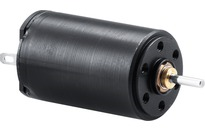
\includegraphics[scale=0.01]{img/motor.png}
\caption{FAULHABER\textsuperscript{\textregistered} 1524T012SR}
\label{fig:motor}
\end{figure} 

Este motor tiene una conmutaci\'{o}n de metales preciosos, esto se refiere a los materiales usados en las escobillas y el conmutador consisten en aleaciones de metales preciosos de alto desempe\~{n}o. Este tipo de sistema de conmutaci\'{o}n es usado principalmente debido a su peque\~{n}o tama\~{n}o, muy baja fricci\'{o}n y una se\~{n}al precisa de conmutaci\'{o}n. En general los motores con conmutaci\'{o}n de metales preciosos exhiben el mejor desempe\~{n}o. Los par\'{a}metros del motor se resumen en la tabla ~\ref{Table:MotorParameters}.

\begin{table}[H]
\caption{Par\'{a}metros del Motor}
\label{Table:MotorParameters}
\begin{center}
\begin{tabular}{ |l|c| }
\hline
 \multicolumn{2}{ |c| }{\textbf{Par\'{a}metros del Motor FAULHABER\textsuperscript{\textregistered} 1524T012SR}} \\
\hline
\textit{Par\'{a}metro} & \textit{Valor} \\
\hline
Voltaje Nominal & 12 v  \\
Resistencia T\'{e}rmica & 19.8 $\Omega$  \\
Potencia de Salida & 1.75 W  \\
Eficiencia M\'{a}xima & 76 \%  \\
Velocidad sin carga & 9900 rpm  \\
Corriente sin carga & 0.011 A  \\
Par de Fricci\'{o}n & 0.13 mNm  \\
Constante de Velocidad & 840 rpm/v \\
Constante de Par & 11.4 mNm/A \\
Constante de Corriente & 0.088 A/mNm \\
Inductancia del Rotor & 250 $\mu$H \\
Constante de Tiempo Mec\'{a}nica & 10 ms \\
Inercia del Rotor & 0.65 g cm\textsuperscript{2}\\
Aceleraci\'{o} Angular & 100x10\textsuperscript{3} rad/s\textsuperscript{2} \\
Peso & 21 g \\
Material Magnetico & NdFeB\\
\hline
\end{tabular}
\end{center}
\end{table}
 

Adicionalmente se ha equipado al motor con un moto-reductor FAULHABER\textsuperscript{\textregistered} serie 15/5 con una caja de engranes de tres etapas y una relaci\'{o}n 21:1 que le a\~{n}ade un par adicional al motor. Tambi\'{e}n tiene un encoder incremental de cuadratura FAULHABER\textsuperscript{\textregistered} IE2-512 acoplado a la flecha del motor, sus caracter\'{i}sticas se muestran en la tabla ~\ref{Table:EncParameters}. Finalmente el arreglo final usado se muestra en la figura ~\ref{fig:ArrMotor}.

\begin{table}[H]
\caption{Caracter\'{i}sticas del Encoder}
\label{Table:EncParameters}
\begin{center}
\begin{tabular}{ |l|c| }
\hline
 \multicolumn{2}{ |c| }{\textbf{Caracter\'{i}sticas del Encoder FAULHABER\textsuperscript{\textregistered} IE2-512}} \\
\hline
\textit{Par\'{a}metro} & \textit{Valor} \\
\hline
Resoluci\'{o}n & 512 PPR  \\
Frecuencia M\'{a}xima & 160 kHz  \\
Voltaje de Alimentaci\'{o}n & 4.5 - 5.5 v  \\
Corriente M\'{a}xima & 13 mA  \\
Desfase ente Canal A y B & 90$^\circ$  \\
Inercia del disco & 0.09 g cm\textsuperscript{2}  \\
\hline
\end{tabular}
\end{center}
\end{table}

\begin{figure}[H]
\centering 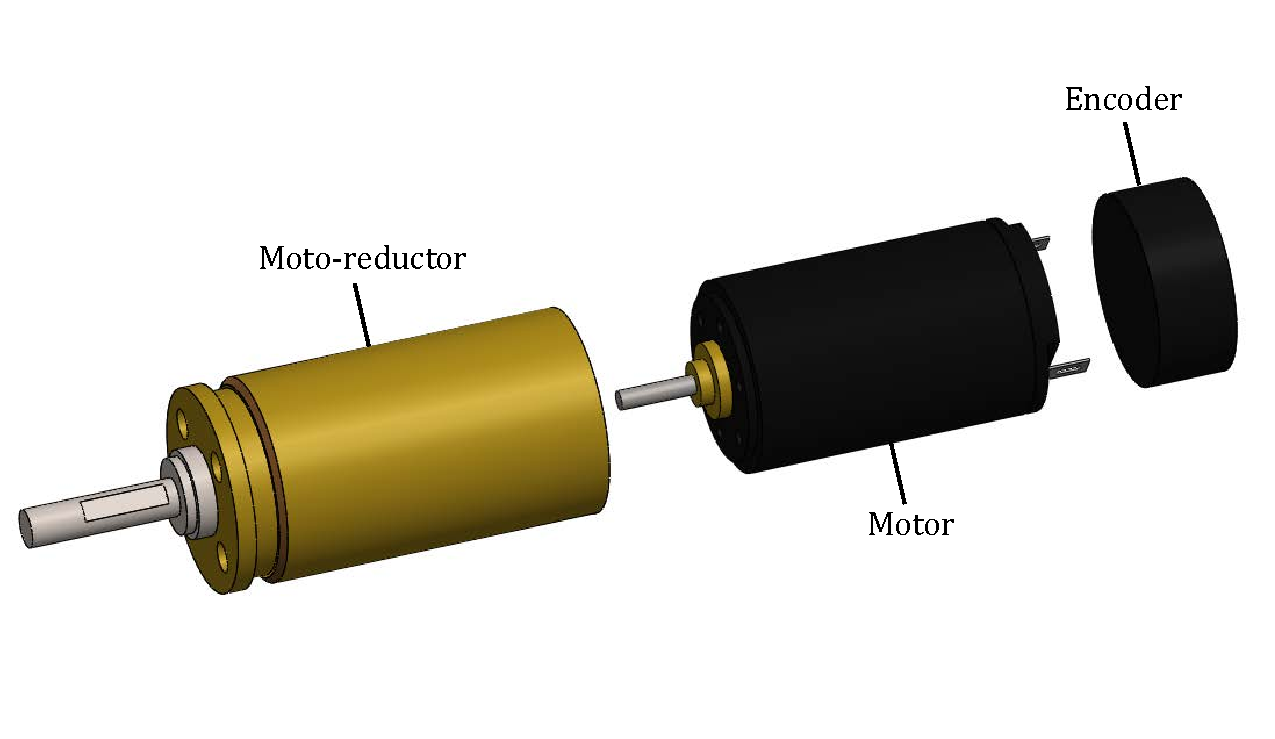
\includegraphics[scale=0.52]{img/ArrMotor.pdf}
\caption{Arreglo Moto-reductor - Motor - Encoder usado en el Sistema}
\label{fig:ArrMotor}
\end{figure}

\subsection{Sensores de l\'{i}mite}

El sistema esta l\'{i}mitado en su rango de movimiento en el eslab\'{o}n interno a 90$^\circ$ debido principalmente al dise\~{n}o de la carcasa, figura ~\ref{fig:LimTilt}. Para asegurar que el sistema \'{u}nicamente trabajar\'{a} en el rango establecido por las l\'{i}mitaciones mec\'{a}nicas se ha dise\~{n}ado un sensor que detecte cuando el \'{a}ngulo de elevaci\'{o}n ha llegado a su l\'{i}mite. Para no a\~{n}adir elementos mec\'{a}nicos extras se ha optado por usar un sensor magn\'{e}tico de efecto Hall para detectar la posici\'{o}n l\'{i}mite de la c\'{a}mara. 

\begin{figure}[H]
\centering 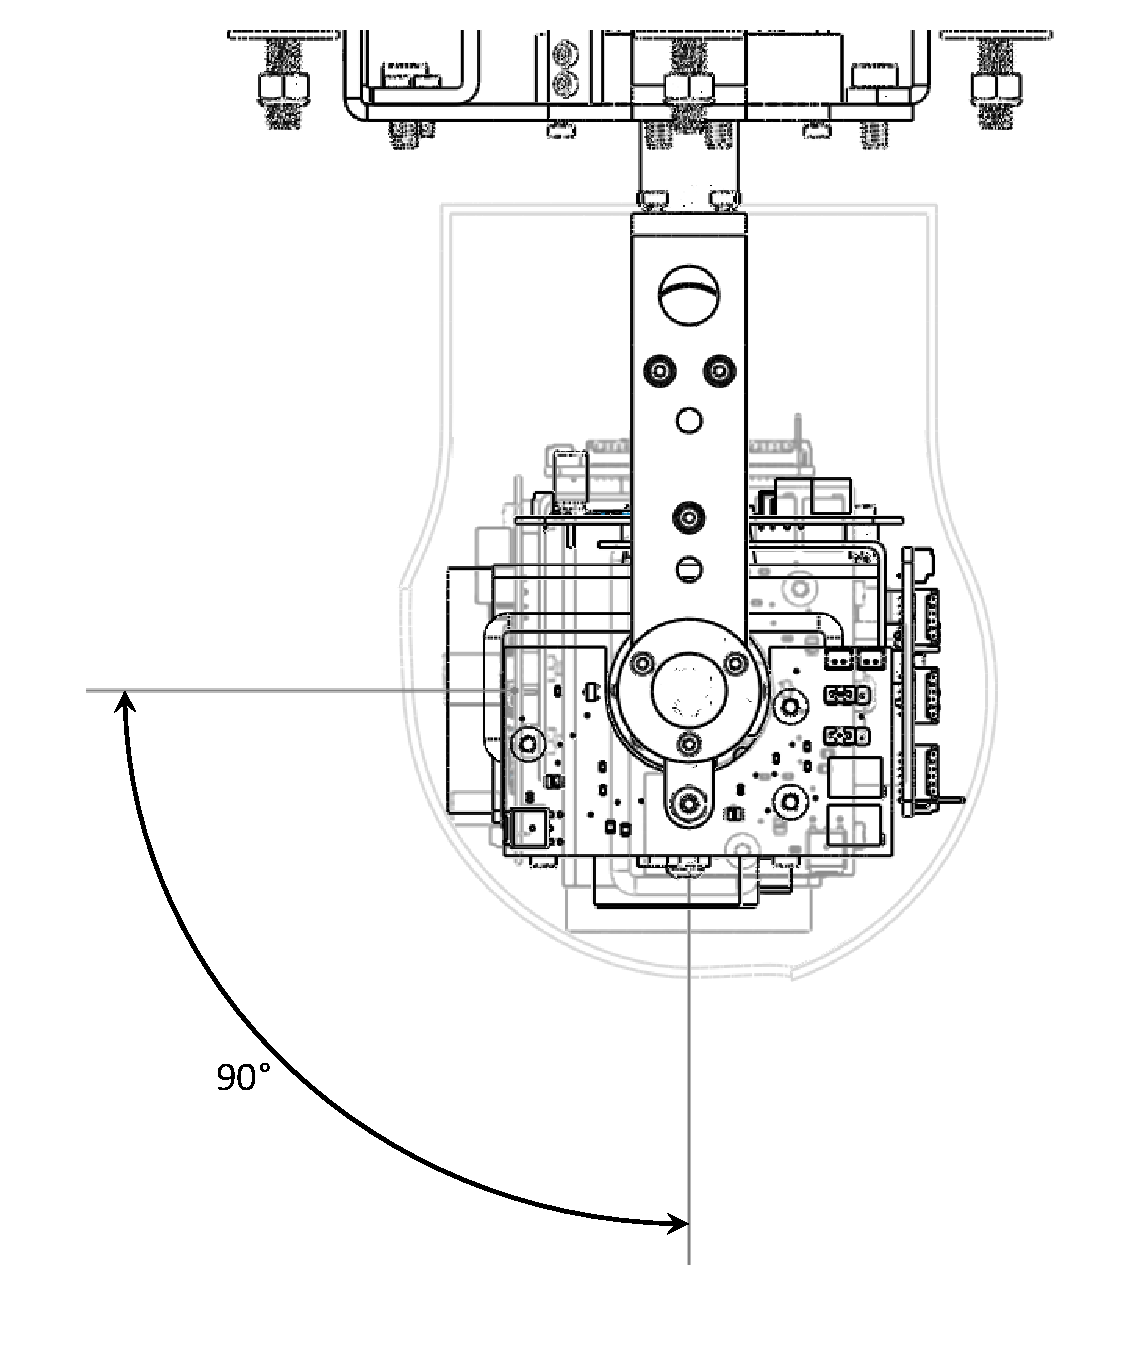
\includegraphics[scale=0.45,trim = 0mm 20mm 0mm 0mm]{img/Limit.pdf}
%trim = izquierda abajo derecha arriba [scale=0.5,trim = 40mm 30mm 110mm 15mm, clip]
\caption{L\'{i}mite Tilt}
\label{fig:LimTilt}
\end{figure} 

Estos sensores se basan en el descubrimiento realizado el Dr. Edwin Hall en 1879, el cual dice que \textit{"Cuando un conductor por que esta circulando una corriente, es expuesto a un campo magn\'{e}tico, se generar\'{a} un voltaje perpendicular a ambos, al flujo de corriente y al campo magn\'{e}tico"}, en su honor se nombro a este el "Efecto Hall", el efecto Hall puede aplicarse a muchos tipos de dispositivos sensores, mientras el par\'{a}metro a medir involucre o pueda involucrar un campo magn\'{e}tico. El voltaje generado por este efecto es muy peque\~{n}o, en el orden de los microvoltios por lo que se requiere de electr\'{o}nica adicional para alcanzar niveles de voltaje pr\'{a}cticos. En el mercado existen dos tipos de sensores efecto Hall: anal\'{o}gicos y digitales, los sensores anal\'{o}gicos proveen una salida anal\'{o}gica de voltaje que es proporcional a la intensidad del campo magn\'{e}tico. La salida de los sensores digitales es discreta, unicamente dos niveles, es decir 1 o 0, nunca en medio y no puede modificarse la magnitud del campo magn\'{e}tico que cambia su estado. Para poder ajustar la precision del sensor, se seleccion\'{o} un sensor de efecto Hall anal\'{o}gico radiom\'{e}trico que provee una salida estable y alta sensibilidad, adem\'{a}s de responder a campos magn\'{e}ticos positivos y negativos. Se dise\~{n}\'{o} la electr\'{o}nica necesaria para el tratamiento de la se\~{n}al, que consiste en un comparador de alta precisi\'{o}n con hist\'{e}resis\footnote{Tendencia de un material a conservar una de sus propiedades, en ausencia del est\'{i}mulo que la ha generado.} ajustable, figura ~\ref{fig:EsqTilt}, este circuito nos permite calibrar de forma precisa la sensibilidad del sensor y producir la se\~{n}al digital que necesita el control.  

\begin{figure}[H]
\centering 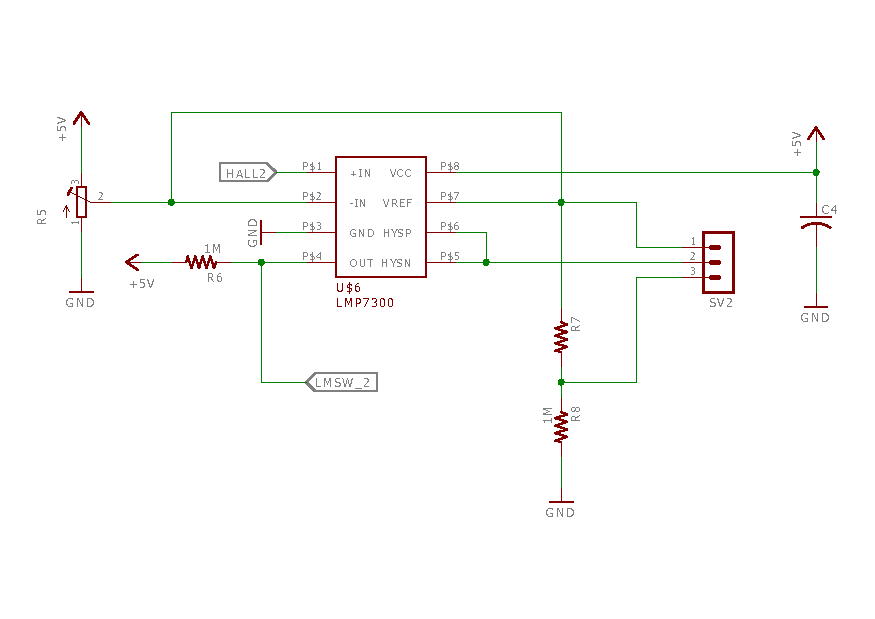
\includegraphics[trim = 0mm 15mm 0mm 15mm]{img/diagram1.pdf}
%trim = izquierda abajo derecha arriba [scale=0.5,trim = 40mm 30mm 110mm 15mm, clip]
\caption{Diagrama Esquem\'{a}tico }
\label{fig:EsqTilt}
\end{figure} 

La tarjeta electronica se dise\~{n}\'{o} usando el programa EAGLE\textsuperscript{\textregistered}, figura ~\ref{fig:CircuitoImp}, integrando el dise\~{n}o mec\'{a}nico del prototipo en el dise\~{n}o electr\'{o}nico para darle una doble funcionalidad a la placa al cuidar la distribuci\'{o}n de los componentes colocando los sensores en la posici\'{o}n necesaria para medir los 90$^\circ$ efectivos de movimiento angular.

\begin{figure}[H]
\centering 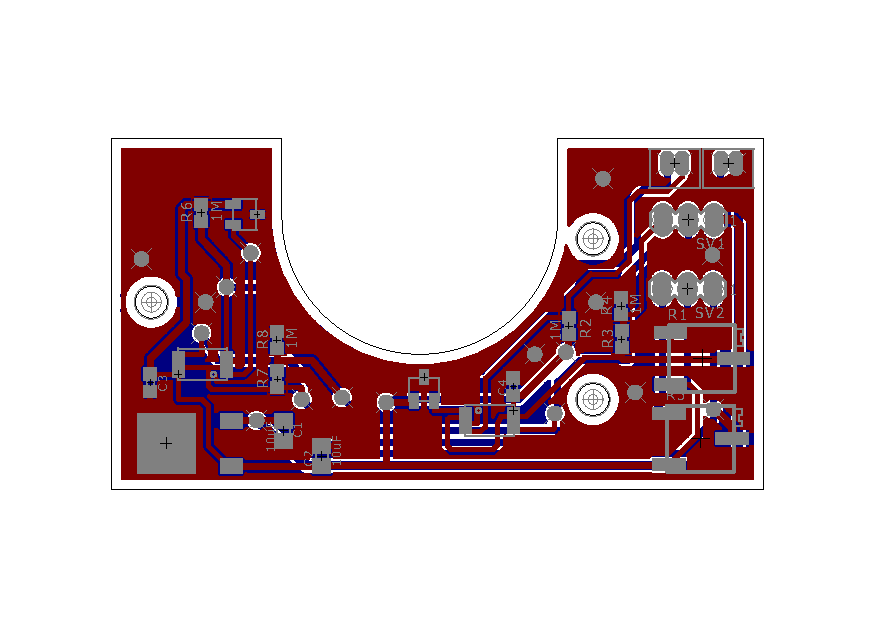
\includegraphics[scale=0.75,trim = 0mm 25mm 0mm 20mm]{img/LimitSW_Tilt_DW_UP.pdf}
%trim = izquierda abajo derecha arriba [scale=0.5,trim = 40mm 30mm 110mm 15mm, clip]
\caption{Dise\~{n}o del Circuito Impreso}
\label{fig:CircuitoImp}
\end{figure} 

Se usaron elementos de montaje superficial para reducir al m\'{a}ximo el tama\~{n}o y el peso del sensor. La forma de placa se ajusta perfectamente para ser montado en el soporte de la c\'{a}mara y la dispoci\'{o}n de los conectores se eligi\'{o} con cuidado para minimizar el uso de cablel El prototipo terminado se muestra en la imagen ~\ref{fig:SenTilt}.

\begin{figure}[H]
\centering 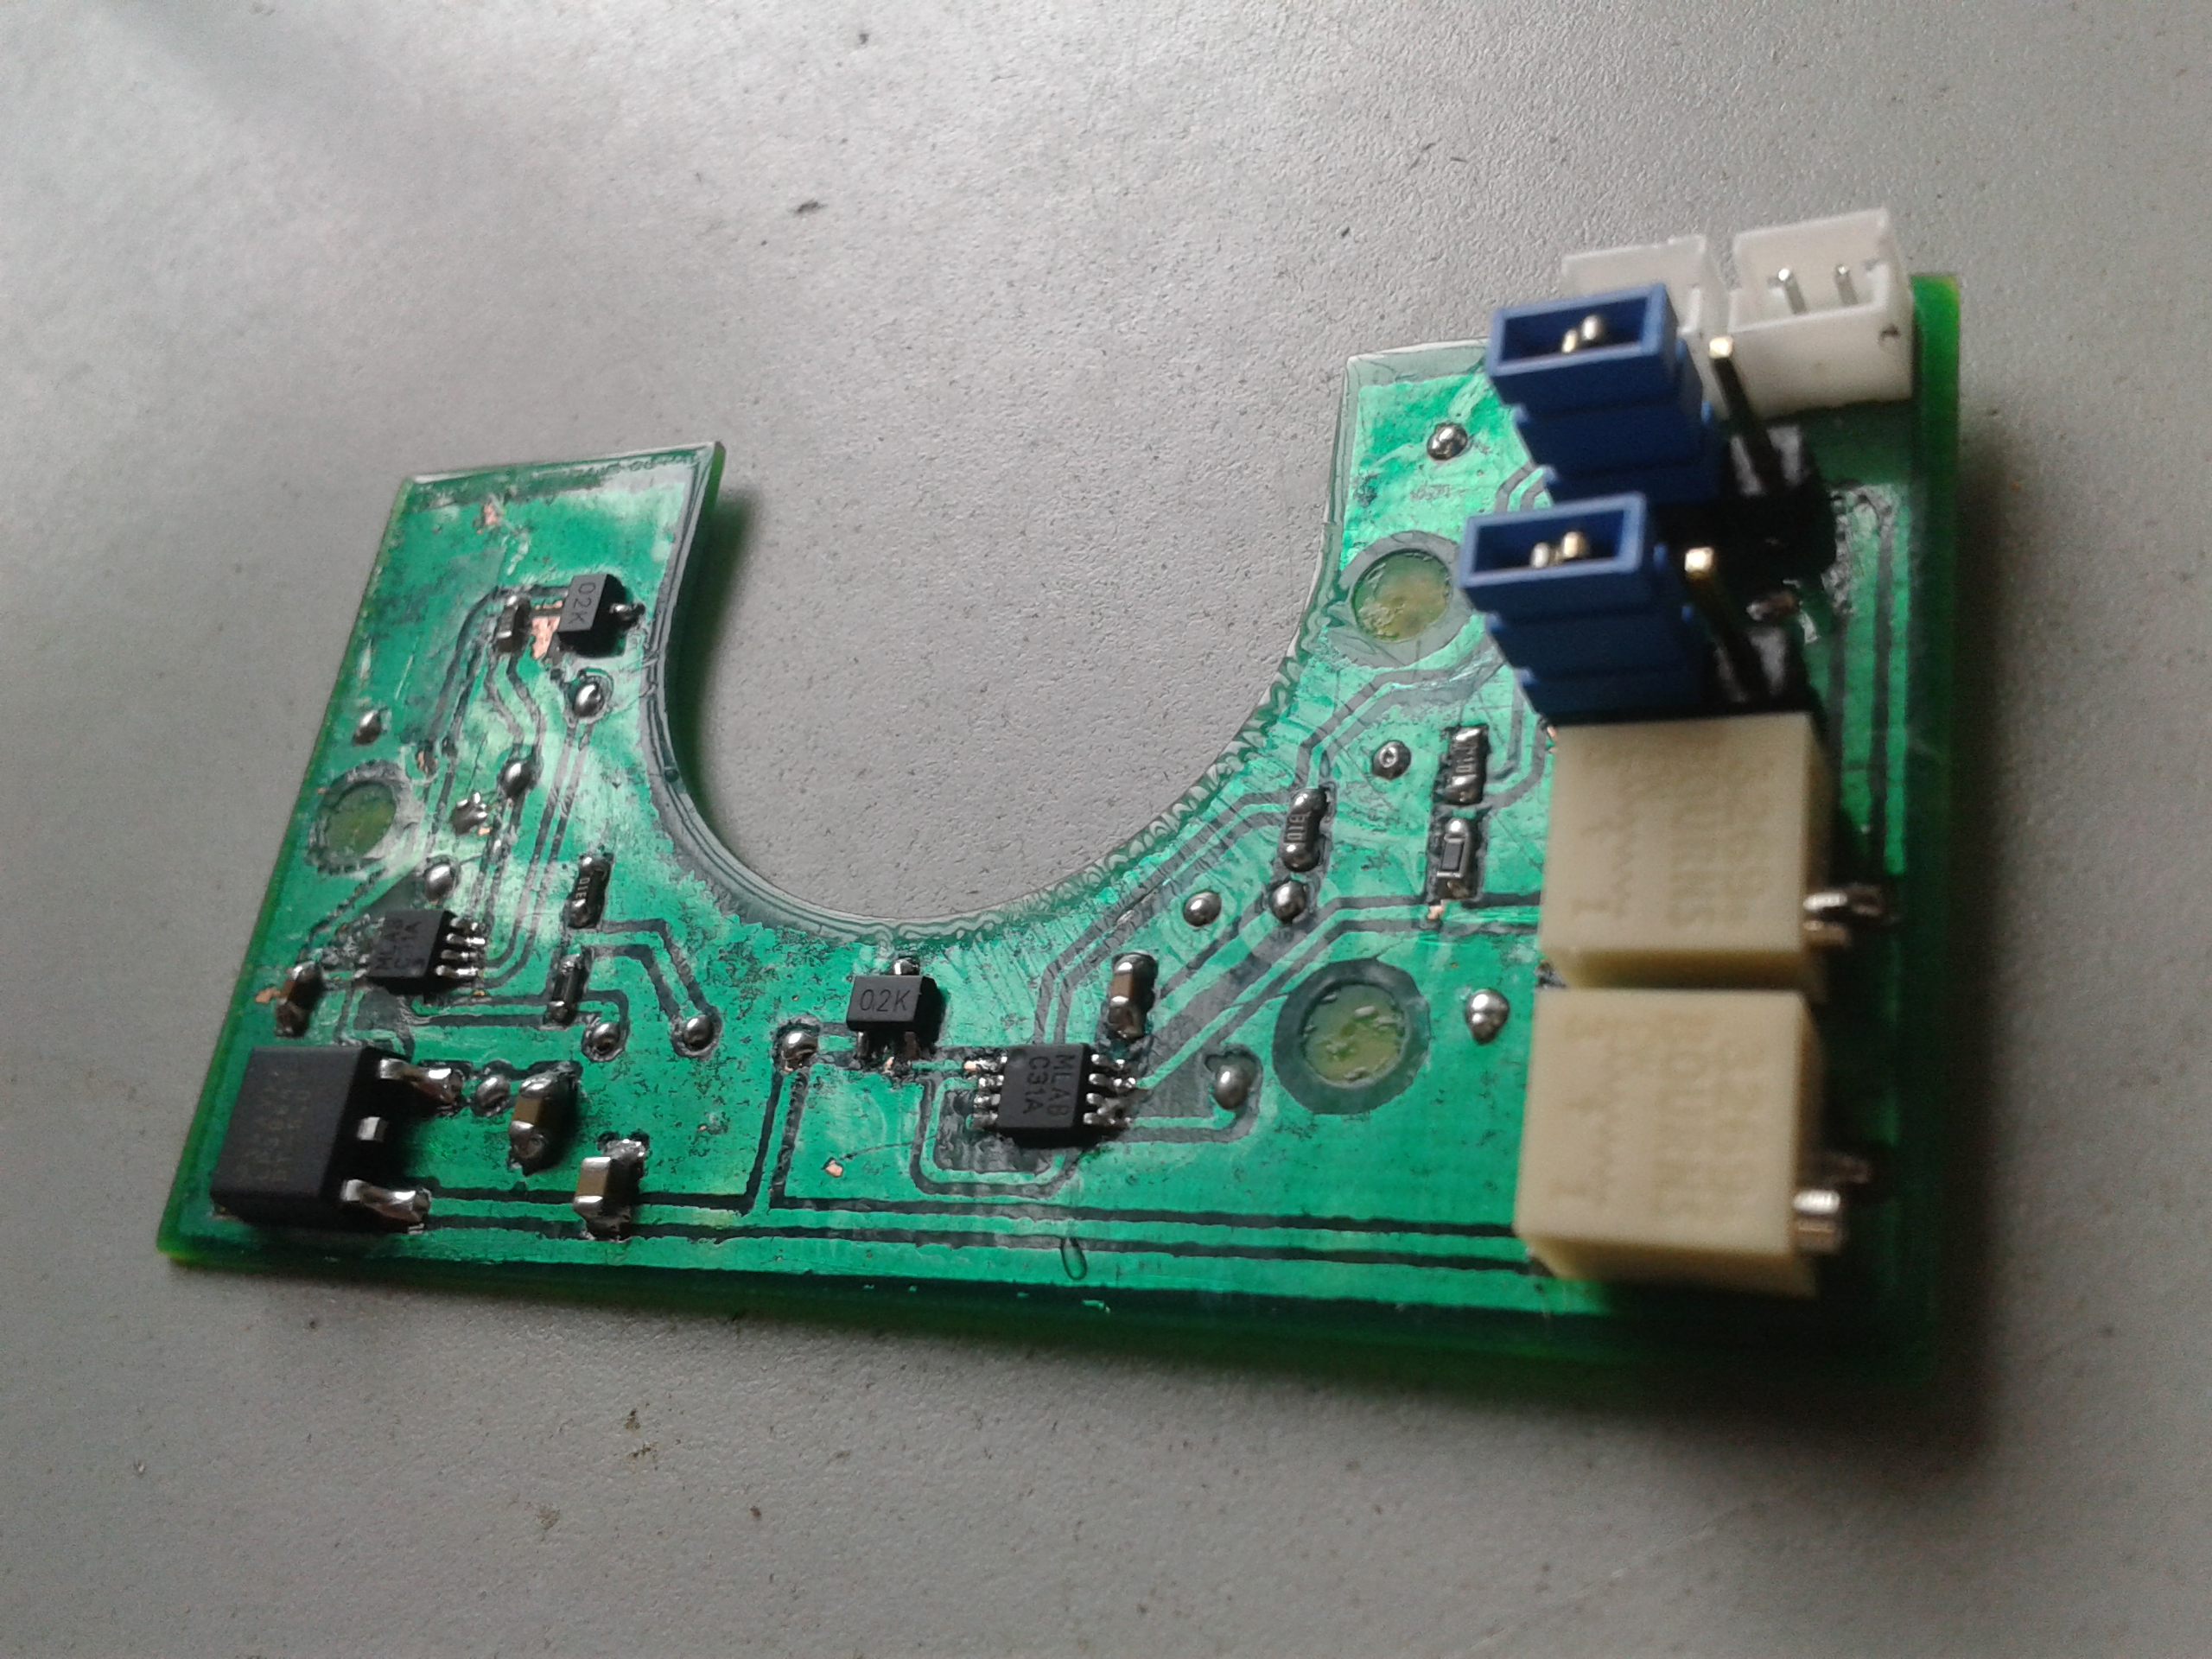
\includegraphics[scale=0.093]{img/SenTilt.jpg}
\caption{Sensor de l\'{i}mite dise\~{n}ado}
\label{fig:SenTilt}
\end{figure} 


Adem\'{a}s de indicar los limites f\'{i}sicos los sensores tienen otra funci\'{o}n importante, la cual es establecer la posici\'{o}n "Home" del sistema, es decir, una ubicaci\'{o}n conocida y fija en el eje de coordenadas del sistema que indique la posici\'{o}n cero para cada eje. La figura ~\ref{fig:HomePos} muestra la posici\'{o}n de los ejes seleccionada para ser la posici\'{o}n cero o "home" del gimbal. 

\begin{figure}[H]
\centering 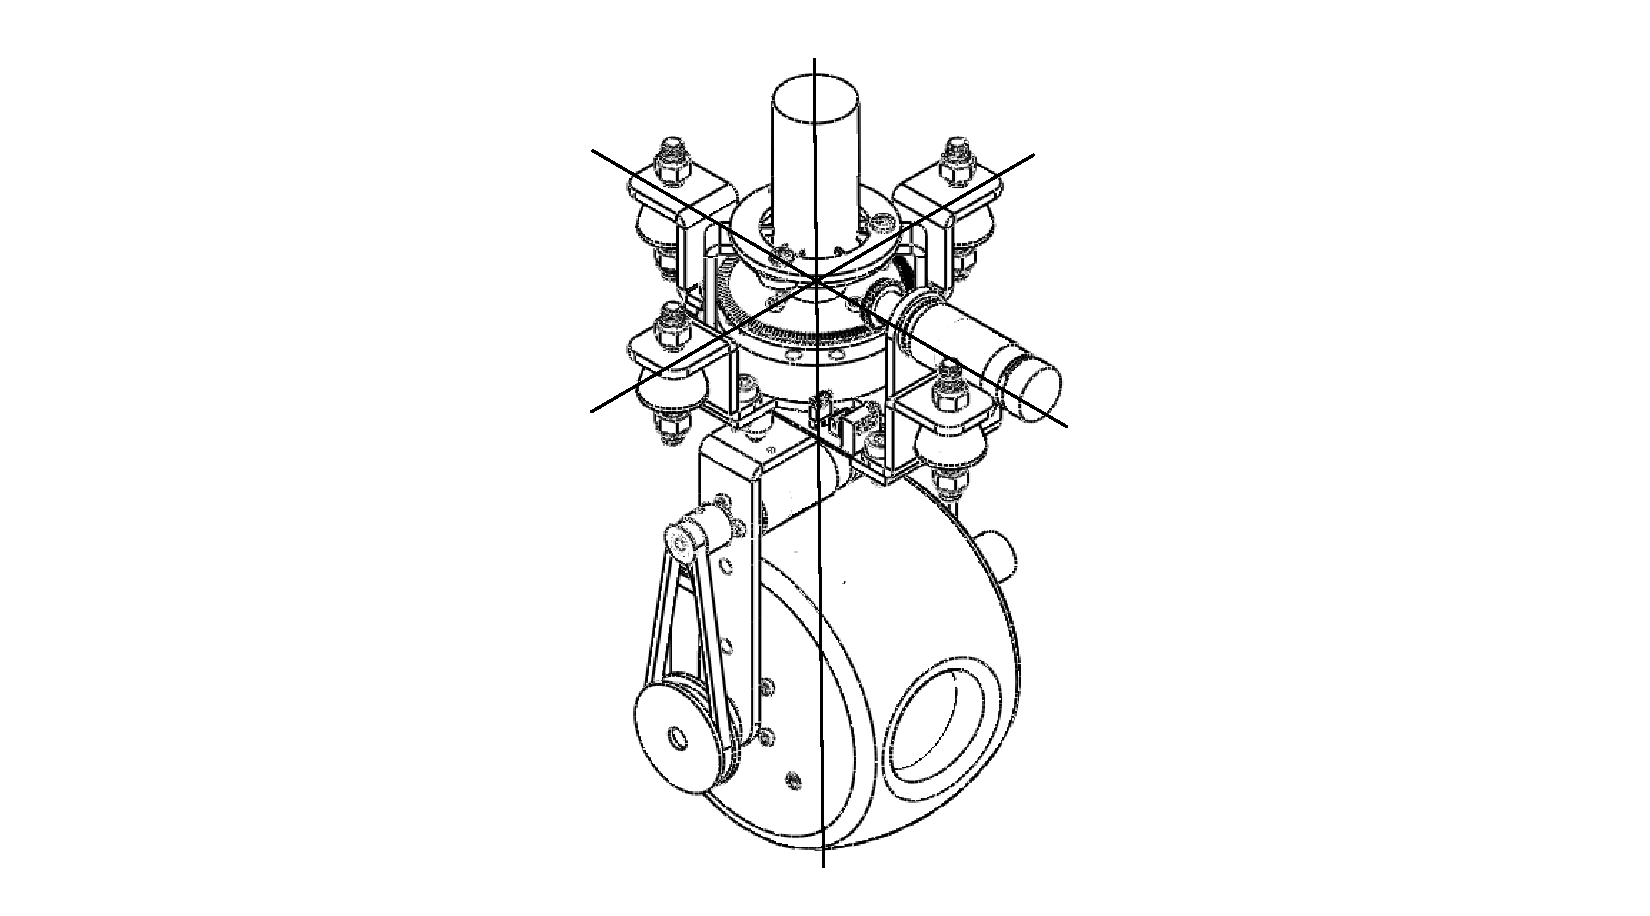
\includegraphics[scale=0.5,trim = 40mm 10mm 40mm 5mm]{img/HomePos.pdf}
%trim = izquierda abajo derecha arriba [scale=0.5,trim = 40mm 30mm 110mm 15mm, clip]
\caption{Posici\'{o}n inicial "Home"}
\label{fig:HomePos}
\end{figure}

Al igual que para el eslab\'{o}n interno se dise\~{n}\'{o} un sensor para el eslab\'{o}n externo. Para este sensor se us\'{o} el mismo sensor radiom\'{e}trico de efecto Hall y el mismo circuito de acondicionamiento. podemos ver el dise\~{n}o de la placa en la figura ~\ref{fig:CircuitoImpPan}.

\begin{figure}[H]
\centering 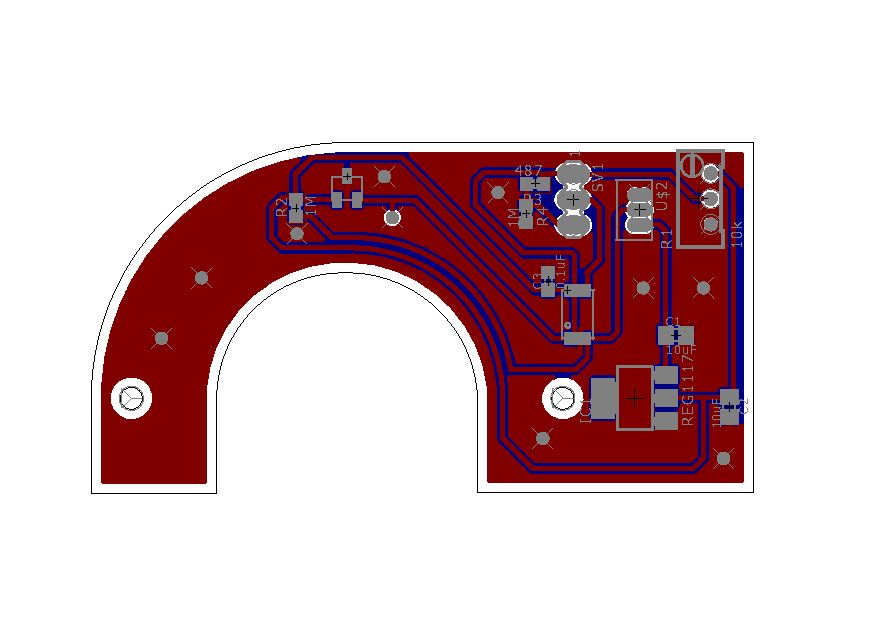
\includegraphics[scale=0.7,trim = 0mm 25mm 0mm 20mm]{img/LimitSW_Pan.pdf}
%trim = izquierda abajo derecha arriba [scale=0.5,trim = 40mm 30mm 110mm 15mm, clip]
\caption{Dise\~{n}o del Circuito Impreso del Sensor de Pan}
\label{fig:CircuitoImpPan}
\end{figure}

Como en el dise\~{n}o anterior se tom\'{o} en cuenta la mec\'{a}nica del gimbal para dise\~{n}ar la electr\'{o}nica. La figura ~\ref{fig:SenPan}, muestra el sensor terminado montado en el la base del gimbal y podemos apreciar el actuador magn\'{e}tico que activar\'{a} el sensor. 

\begin{figure}[H]
\centering 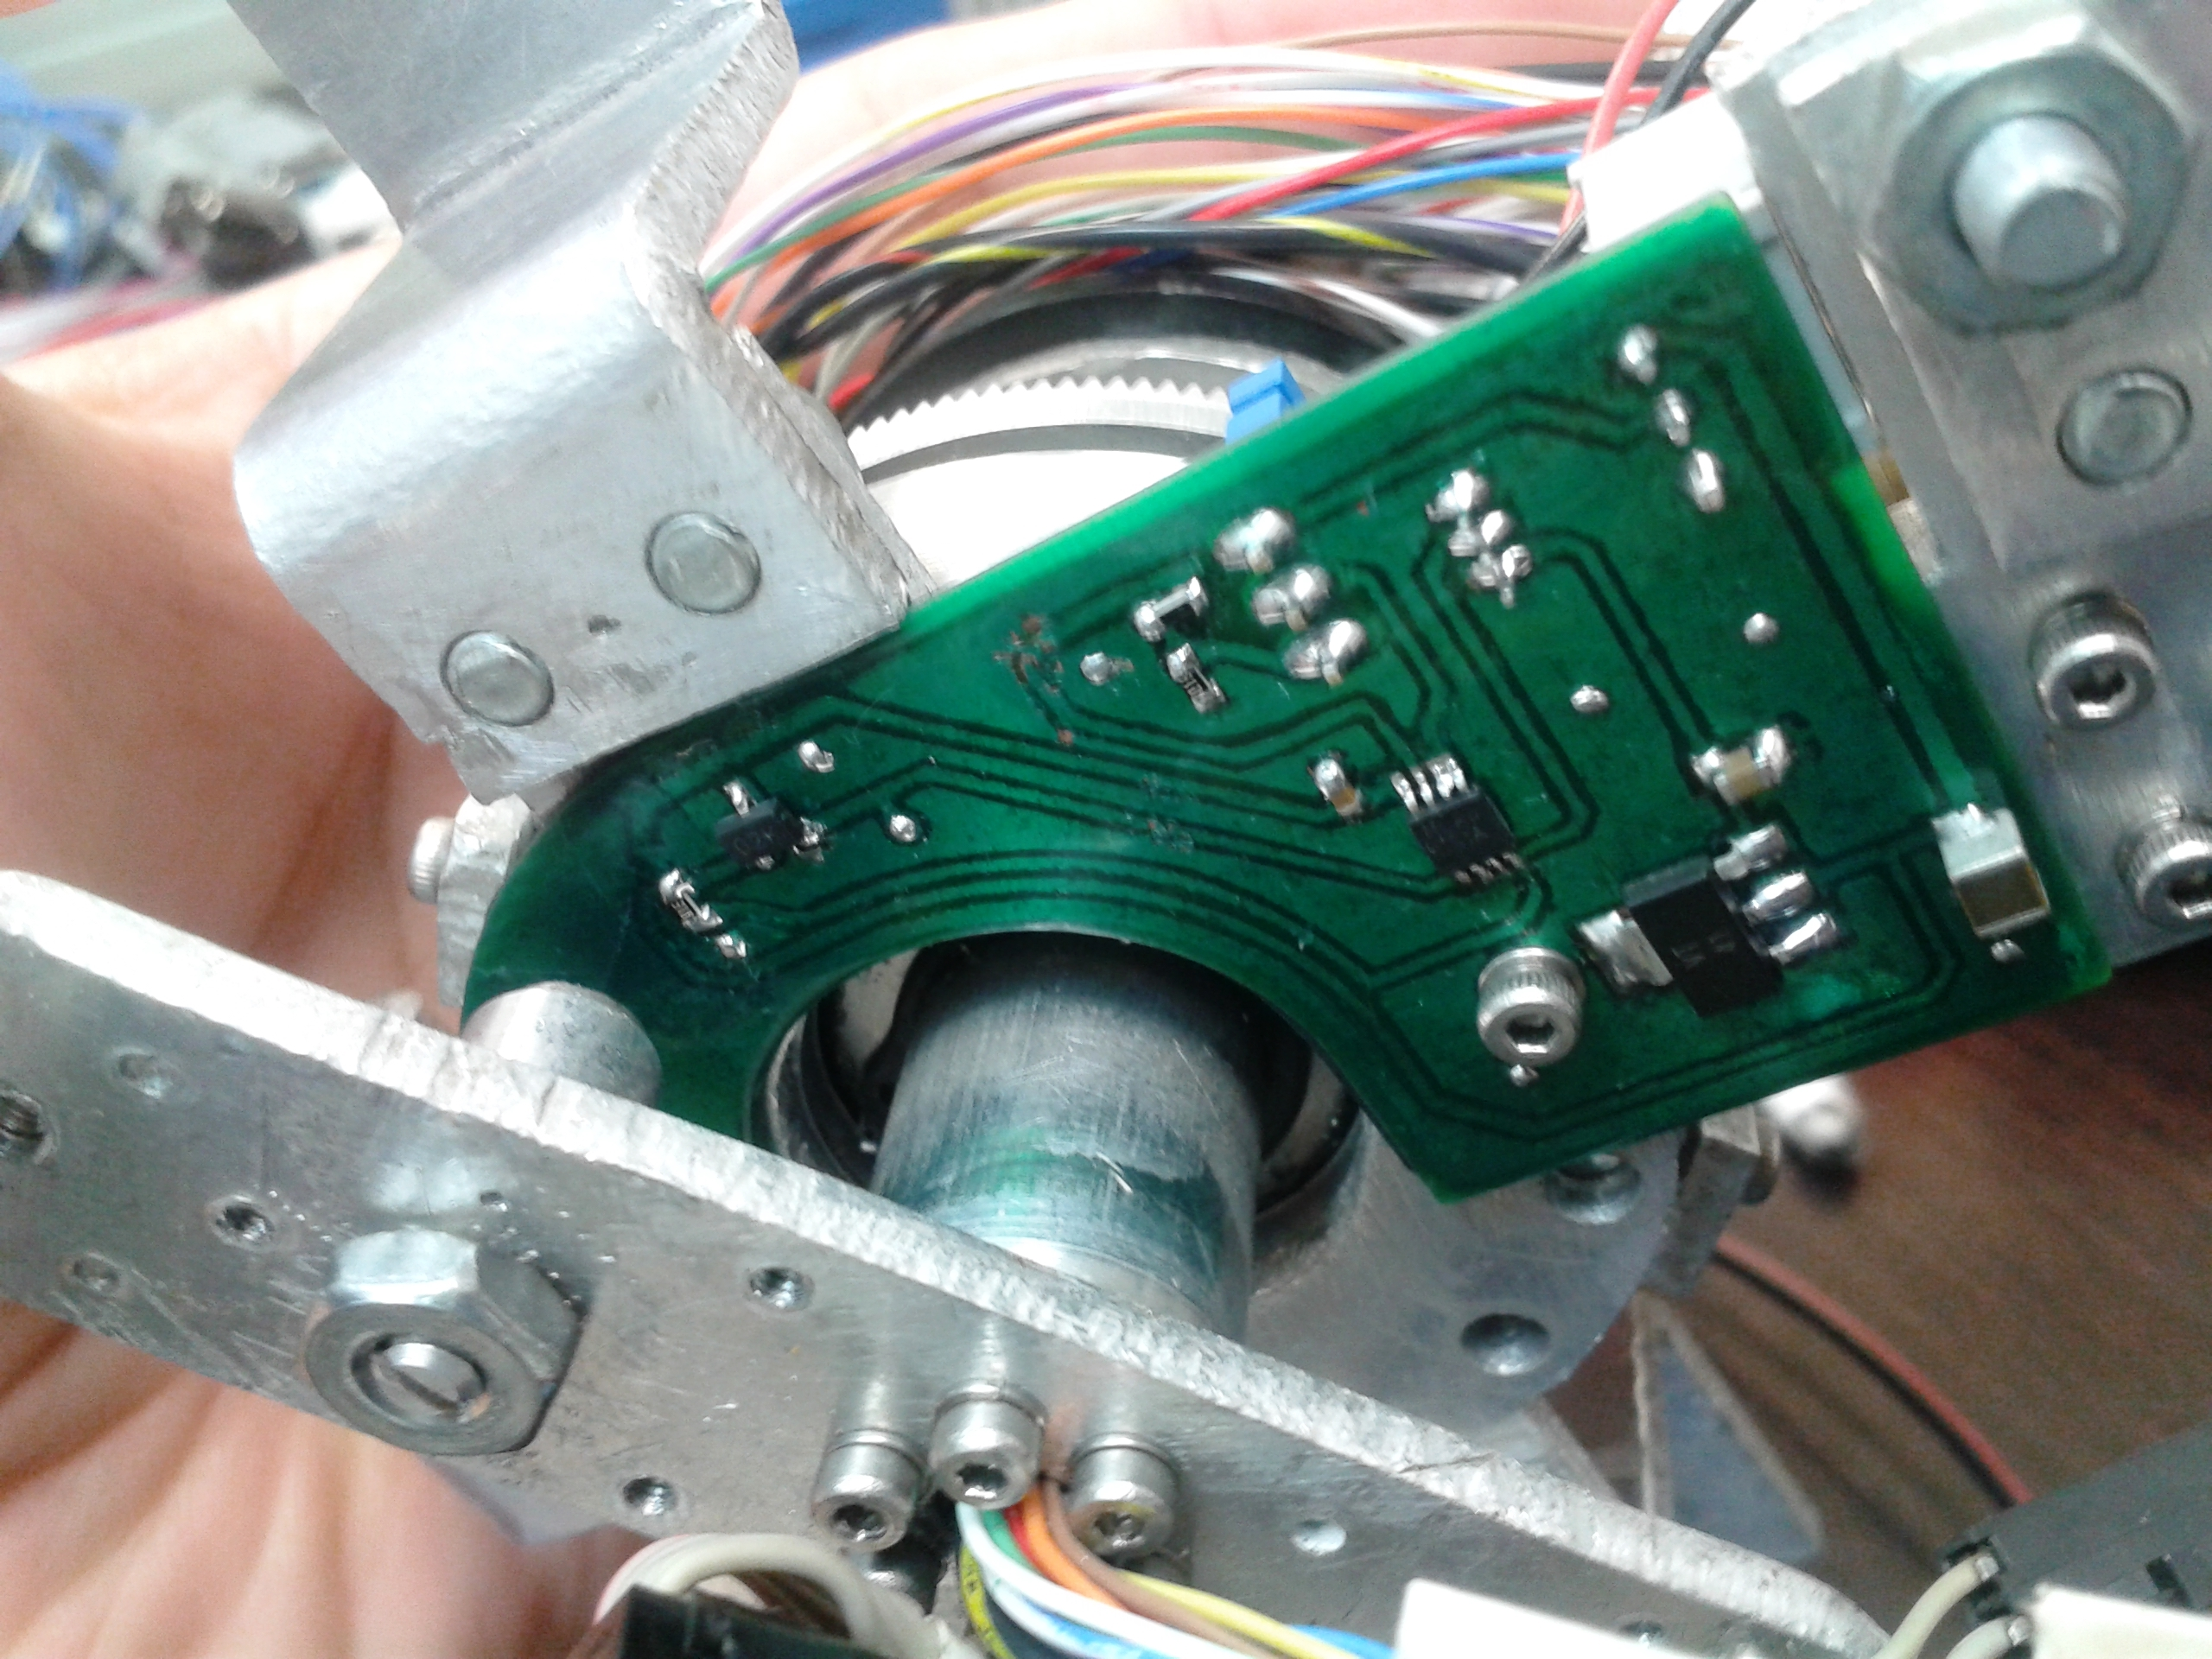
\includegraphics[scale=0.093]{img/SenPan.jpg}
\caption{Sensor de l\'{i}mite Dise\~{n}ado Montado en el Prototipo}
\label{fig:SenPan}
\end{figure}

  
\section{Mec\'anica}

\subsection{Estructura Principal}

La estructura mec\'{a}nica del prototipo consta principalmente de tres partes, la base, la cual permite el montaje del sistema en la aeronave, el eslab\'{o}n externo, el cual permite el movimiento en acimut del sensor  y finalmente el eslab\'{o}n interno el cual permite el movimiento en tilt del sensor. El material utilizado es aluminio 6160, el cual es una aleaci\'{o}n de aluminio endurecido que contiene como principales elementos aluminio, magnesio y silicio.  Tiene buenas propiedades mec\'{a}nicas y es usado generalmente para la construcci\'{o}n de estructuras de aeronaves como las alas y el fuselaje de aviones comerciales y de uso militar \cite{28}. 

La base tiene la funci\'{o}n de fijar el sistema en la plataforma a\'{e}rea, podemos observar a detalle el dise\~{n}o de la base en la figura ~\ref{fig:Base}, esta permite la fijaci\'{o}n del prototipo por medio de cuatro amortiguadores vibratorios que reducen el efecto de las vibraciones sobre el sistema, tambi\'{e}n tiene el motor y la transmici\'{o}n para mover el eslab\'{o}n externo. Para poder transmitir las se\~{n}ales se us\'{o} un slip ring para permitir una rotaci\'{o}n de 360 grados entre la base y el eslab\'{o}n externo.

\begin{figure}[H]
\centering 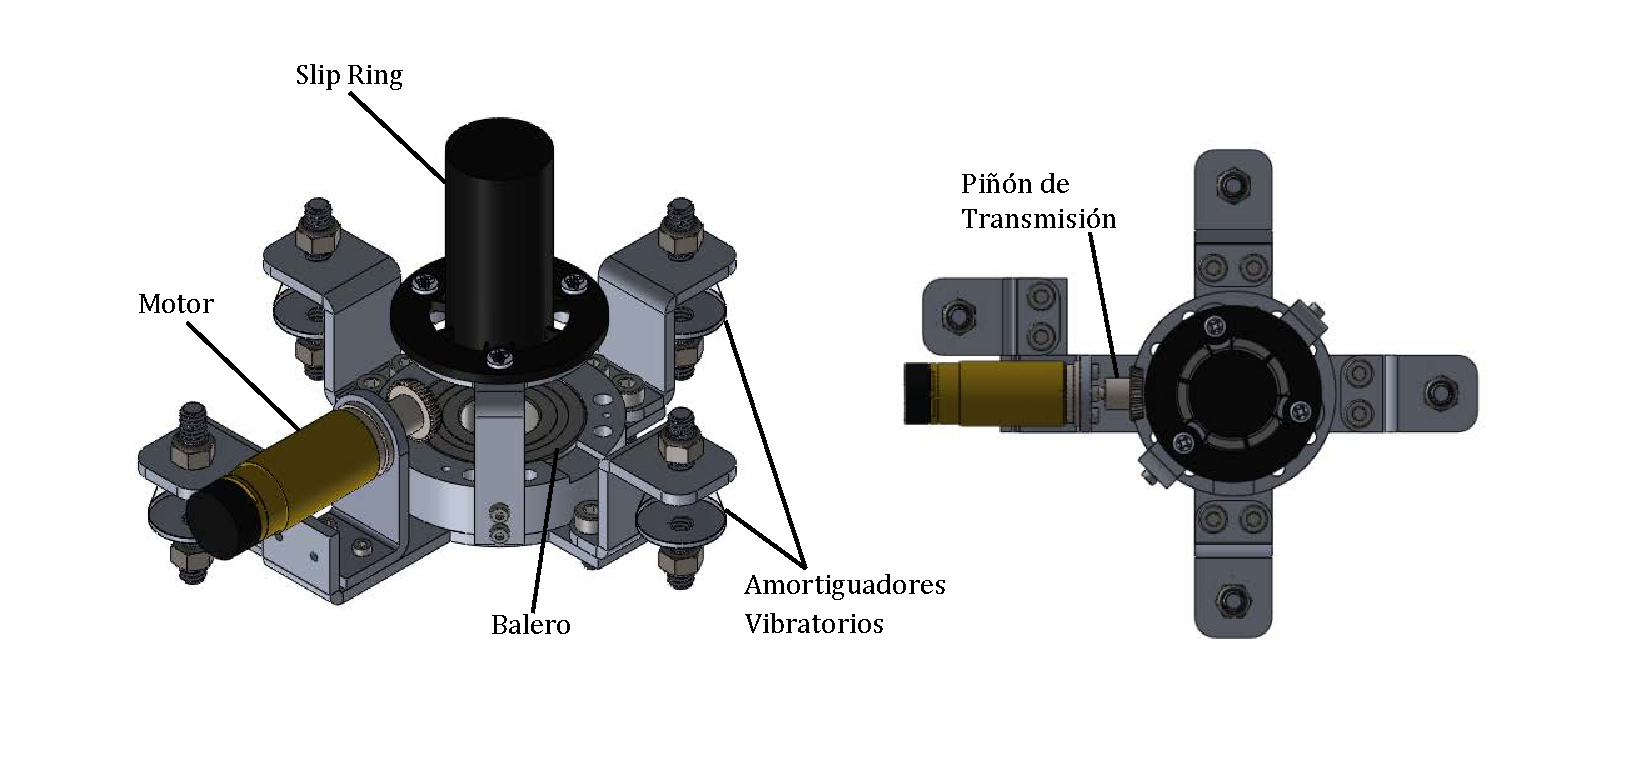
\includegraphics[scale=0.55,trim = 30mm 20mm 30mm 5mm]{img/BaseGimbal.pdf}
%trim = izquierda abajo derecha arriba [scale=0.5,trim = 40mm 30mm 110mm 15mm, clip]
\caption{Detalle de la Estructura de la Base y Montaje del Gimbal}
\label{fig:Base}
\end{figure}

La estructura del eslab\'{o}n externo se muestra en la figura ~\ref{fig:Pan}, en esta imagen podemos observar que consta de un eje al cual se transmite el movimiento a trav\'{e}s de un sistema de corona-pi\~{n}on a la estructura en forma de u que sostendr\'{a} al eslab\'{o}n interno. Este eje esta hueco para que los cables que transmiten las se\~{n}ales desde y hacia la tarjeta principal de control puedan llegar a la tarjeta de control de tilt, estas se\~{n}ales pasan por un dispositivo slip ring tal como se mencion\'{o} anteriormente para permitir un giro completo entre la base y el eslab\'{o}n externo. En esta estructura esta montado el motor que mueve el eslab\'{o}n interno por medio de una transmisi\'{o}n tipo banda. Para poder transmitir las se\~{n}ales hasta la tarjeta de control en tilt, se instal\'{o} un segundo slip ring entre el eslab\'{o}n externo y el interno que tambi\'{e}n podemos apreciar en la figura ~\ref{fig:Pan}, esto permite que el eslab\'{o}n interno pueda realizar giros completos y elimina las restricciones provocadas por los cables. Hay un magneto montado en el eslab\'{o}n externo que sirve como actuador al sensor de l\'{i}mite el cual funciona para calibraci\'{o}n del encoder para medir el \'{a}ngulo entre la base y el eslab\'{o}n externo. 


\begin{figure}[H]
\centering 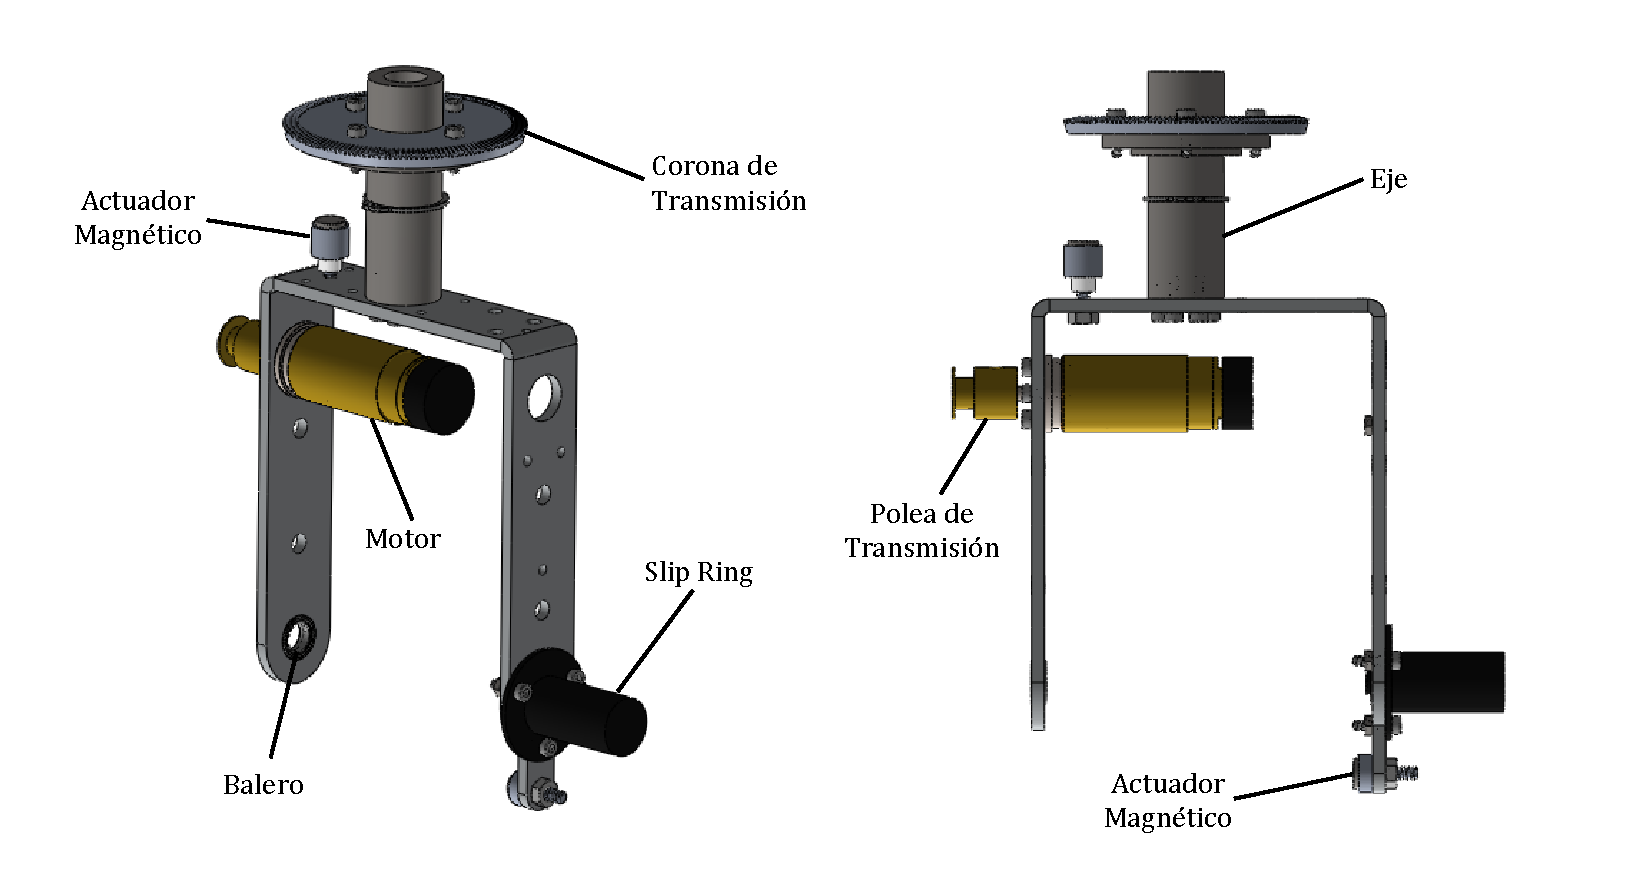
\includegraphics[scale=0.53,trim = 30mm 5mm 30mm 10mm]{img/BasePan.pdf}
%trim = izquierda abajo derecha arriba 
\caption{Detalle de la Estructura del Eslab\'{o}n Externo (Pan)}
\label{fig:Pan}
\end{figure}

La estructura principal del eslab\'{o}n interno se muestra en la figura ~\ref{fig:Tilt}. Este consta de dos ejes de aluminio 6160 y un soporte para la c\'{a}mara fabricado en fibra de vidrio. La transmisi\'{o}n es por medio de una polea y este arreglo permite girar la c\'{a}mara sobre el eje \textit{y} y el montaje de todos los elementos necesarios para el funcionamiento del sistema, es decir, la c\'{a}mara, la central inercial y la tarjeta de control. 


\begin{figure}[H]
\centering 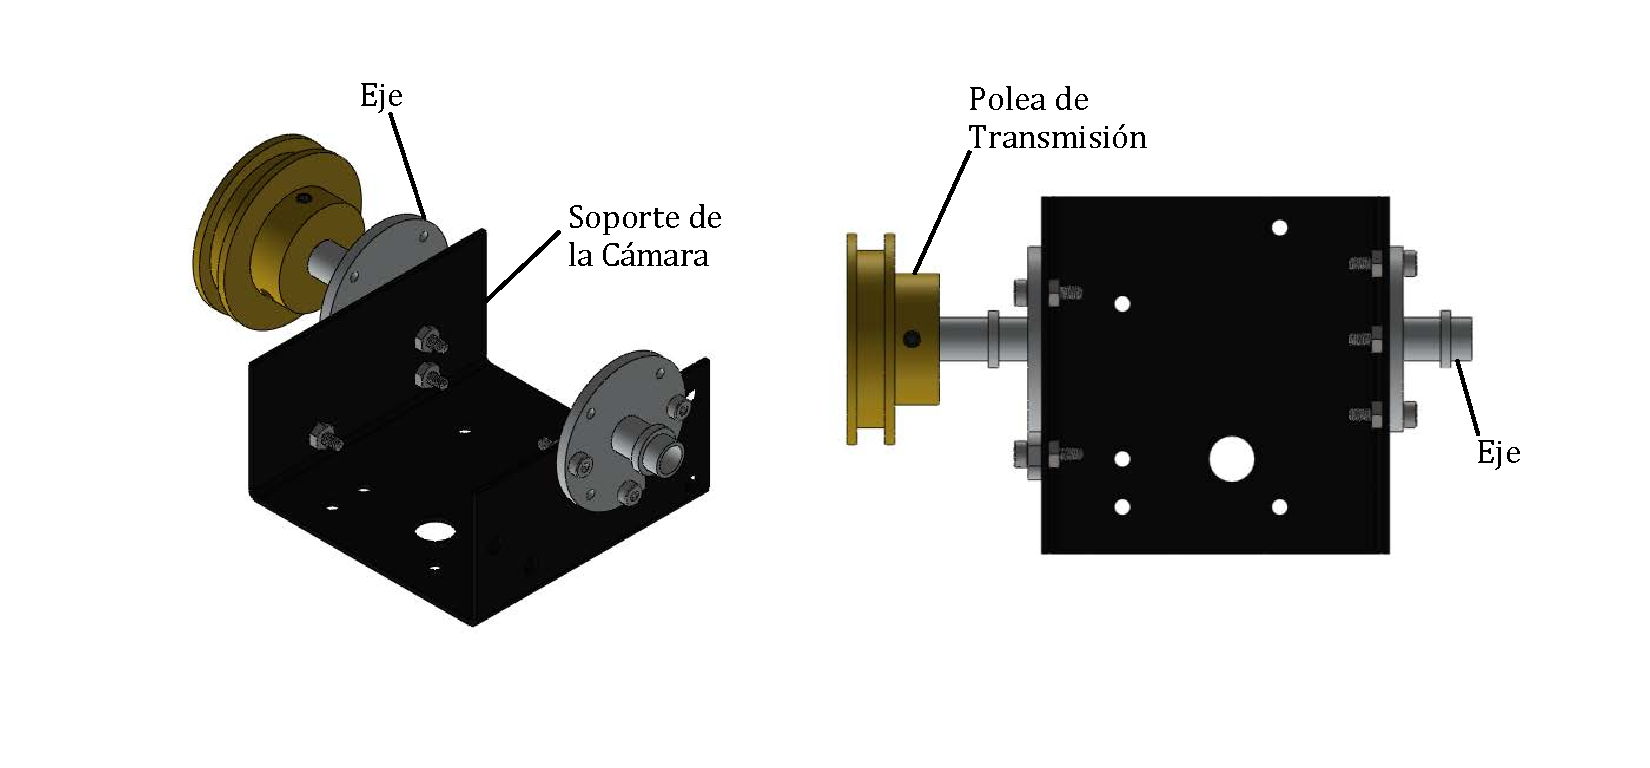
\includegraphics[scale=0.47,trim = 30mm 25mm 20mm 5mm]{img/BaseTilt.pdf}
%trim = izquierda abajo derecha arriba 
\caption{Detalle de la Estructura del Eslab\'{o}n Interno (Tilt)}
\label{fig:Tilt}
\end{figure} 


\section{Programaci\'{o}n}\label{sec:Programacion}

\subsection{Introducci\'{o}n}

\textit{MPLAB\textsuperscript{\textregistered} Device Blocks for Simulink\textsuperscript{\textregistered}} es una tecnolog\'{i}a desarrollada por la empresa Microchip\textsuperscript{\textregistered} que consiste en un juego de bloques que se integra con el ambiente de MATLAB\textsuperscript{\textregistered}/Simulink\textsuperscript{\textregistered} para extender sus capacidades y funciones, los bloques a\~{n}adidos permiten configurar f\'{a}cilmente alrededor de 200 diferentes microcontroladores Microchip \textsuperscript{\textregistered} de las familias dsPIC\textsuperscript{\textregistered}30 y dsPIC\textsuperscript{\textregistered}33. Adicionalmente a los bloques, el \textit{MPLAB\textsuperscript{\textregistered} Device Blocks for Simulink\textsuperscript{\textregistered}} a\~{n}ade codigos a MATLAB que permite programar el microcontrolador y conectarlo a trav\'{e}s  de un puerto serial para analizar los datos. Si bien Simulink y MATLAB son capaces de generar c\'{o}digo C, este paquete adicional permite generar un c\'{o}digo C compatible con el microcontrolador, las tareas que realiza durante el proceso de generaci\'{o}n del c\'{o}digo son las siguientes:    

\begin{itemize}
    \item A\~{n}adir el c\'{o}digo necesario para la configuraci\'{o}n del microcontrolador especifico.
    \item A\~{n}adir el c\'{o}digo necesario para configurar los perif\'{e}ricos usados.
    \item A\~{n}adir el c\'{o}digo del gestionador de tareas.
    \item Compilar el c\'{o}digo global generado para obtener un archivo binario listo para grabar (.cof,
.hex, o .elf).
\end{itemize}

Adicionalmente, crea un proyecto MPLAB X IDE\footnote{Software de programaci\'{o}n para desarrollar aplicaciones para microcontroladores y controladores digitales de se\~{n}ales Microchip\textsuperscript{\textregistered}. Es llamado in Entorno de Desarrollo Integrado (IDE), ya que provee un \'{u}nico entorno integrado para desarrollar c\'{o}digo para microcontroladores embarcados} en donde podemos ver el c\'{o}digo generado.


\subsection{Programaci\'{o}n por Bloques}

En la figura ~\ref{fig:ProgDiag} se muestra uno de los algoritmos programados usando el \textit{MPLAB\textsuperscript{\textregistered} Device Blocks for Simulink\textsuperscript{\textregistered}}. El bloque principal es el "Microchip Master" Este bloque corrobora y corrige los par\'{a}metros de Simulink para cumplir con las restricciones de generaci\'{o}n de c\'{o}digo, adem\'{a}s en este bloque se definen los par\'{a}metros esenciales relacionados con el microcontrolador seleccionado. Por defecto, Simulink est\'{a} preconfigurado con un solucionador continuo que permite  la simulaci\'{o}n ya sea para un modelo continuo, discreto o una mezcla de ambos, tiempo continuo y discreto. Para la generaci\'{o}n de c\'{o}digo se requiere que la configuraci\'{o}n de Simulink sea con el uso de un solucionador de tiempo discreto, cuando se coloca un bloque "Microchip Master" las configuraciones del solucionador se hacen autom\'{a}ticamente.  

\begin{figure}[H]
\centering 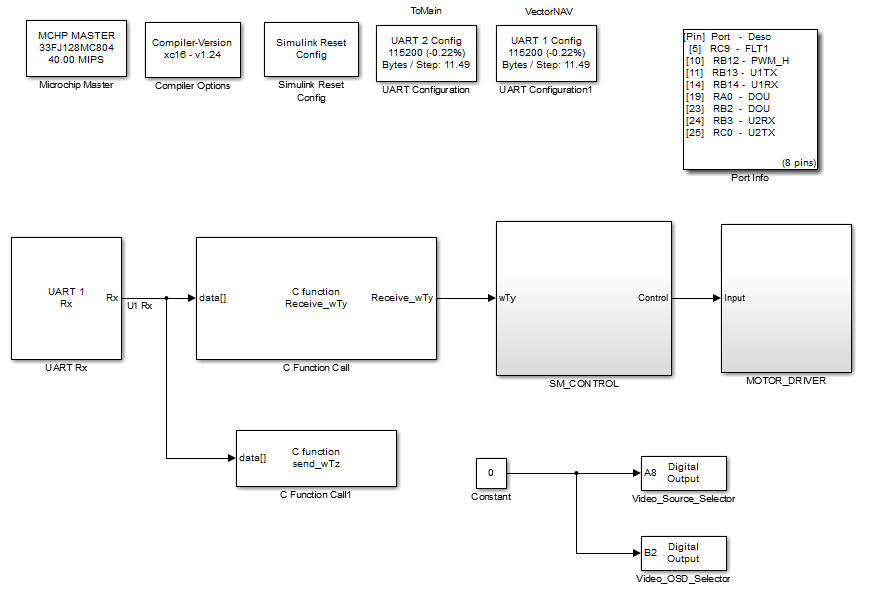
\includegraphics[scale=0.65]{img/DiaProg.png}
\caption{Diagrama de Bloques del Programa del Algoritmo de Estabilizaci\'{o}n}
\label{fig:ProgDiag}
\end{figure}

El bloque \textit{Compiler Option} permite seleccionar el compilador y algunas opciones de compilaci\'{o}n. En este se listan todos los compiladores instalados en el sistema pero no se realiza una prueba de compatibilidad con el dispositivo elegido, por lo que hay que revisar en la documentaci\'{o}n del microcontrolador seleccionado, cual es el compilador compatible. El bloque \textit{Reset Config} revisa que la configuraci\'{o}n de Simulink sea correcta y se usa cuando se trabaja en diferentes computadoras pues permite corregir la ruta de los archivos para la compilaci'{o}n. El bloque \textit{Port info} muestra una relaci\'{o}n de los pines usados en el dispositivo y el perif\'{e}rico al que pertenecen, es muy \'{u}til pues la mayor\'{i}a de los dispositivos soportados tienen pines remapeables por lo que es una ayuda visual para corroborar que la configuraci\'{o}n de los pines corresponde con la capa f\'{i}sica del circuito. El bloque \textit{Digital Output} configura los pines como salidas digitales y permite la escritura en el estado del pin. La entrada del bloque corresponde con la salida digital seleccionada. Un bloque puede configurar \'{u}nicamente un puerto, por ejemplo PORTA o PORTB, pero para el puerto seleccionado pueden configurarse varios pines, cuando se selecciona m\'{a}s de un pin con un bloque, existe la opci\'{o}n para que la actualizaci\'{o}n del estado sea simultanea o de lo contrario la actualizaci\'{o}n ser\'{a} en secuencia. El bloque \textit{UART Configuration} configura el perif\'{e}rico UART elegido: Este bloque permite la configuraci\'{o}n de la velocidad de transmisi\'{o}n  y elegir los pines Rx y Tx. Este bloque permite tambi\'{e}n elegir entre varios tipos de implementaci\'{o}n para la recepci\'{o}n de datos por la comunicaci\'{o}n serial:

 
\begin{itemize}
    \item Solo el buffer\footnote{Es un espacio de memoria, en el que se almacenan datos de manera temporal} interno de 4 bytes.
    \item Buffer Circular.
    \item Modo DMA Ping-Pong.
    \item DMA usando un solo buffer.
\end{itemize}

Las opciones de implementaci\'{o}n DMA solo estan disponibles para los dispositivos que soporten el uso de DMA. Para el modo DMA Ping-Pong, se inicializan dos buffers y se llenan en secuencia. El primer buffer se env\'{i}a hasta que esta completamente lleno. En el modo DMA de un solo buffer, solo se inicializa un buffer y tiene el inconveniente de poder presentar perdida de datos. El bloque \textit{C Function Call} permite incluir c\'{o}digo en lenguaje C dentro del proyecto de Simulink. Estos archivos C ser\'{a}n utilizados para la generaci\'{o}n de c\'{o}digo y permiten la utilizaci\'{o}n de registros e instrucciones especificas del dispositivo. El archivo del c\'{o}digo en C debe declararse en los par\'{a}metros de configuraci\'{o}n de Simulink en el men\'{u} de generaci\'{o}n de c\'{o}digo para a\~{n}adir la ruta del archivo al directorio de Simulink.

En conclusi\'{o}n el \textit{MPLAB\textsuperscript{\textregistered} Device Blocks for Simulink\textsuperscript{\textregistered}}, nos permite traducir nuestro modelo de tiempo discreto en su equivalente binario, implementando tambi\'{e}n c\'{o}digo personalizado para aumentar las funciones de los bloques, gracias a esto el n\'{u}mero de iteraciones entre la simulaci\'{o}n y la implementaci\'{o}n se reducen considerablemente y permite probar el algoritmo desarrollado en el prototipo aprovechando las habilidades en el manejo del entorno Simulink sin necesidad de un extensivo y avanzado conocimiento de microcontroladores.






